%TCIDATA{LaTeXparent=0,0,relatorio.tex}
\ifx\compilewholereport\undefined
	\documentclass[11pt,a4paper,oneside]{book}
	
	% Escolher um dos seguintes formatos:
	\usepackage{ft2unb} % segue padrão de fontes do Latex
	
	% Pacotes
	\usepackage{graphicx}
	\usepackage{amsfonts}
	\usepackage{amsmath}
	\usepackage{amssymb}
	\usepackage[thmmarks,amsmath]{ntheorem}
	\usepackage{boxedminipage}
	\usepackage{theorem}
	\usepackage{fancybox}
	\usepackage{fancyhdr}
	\usepackage{url}
	\usepackage{afterpage}
	\usepackage{xcolor}
	\usepackage{rotating}
	\usepackage{makeidx}
	\usepackage{indentfirst}
	\usepackage{subcaption}
	\usepackage{todonotes}
	\usepackage{listings}
	\presetkeys{todonotes}{inline}{}
	
	\begin{document}
	\frontmatter
	\tableofcontents
	\mainmatter
	
	%%%%%%%%%%%%%%%%%%%%%%%%%%%%
	%%%%%%%% Apagar coisas acima
	%%%%%%%%%%%%%%%%%%%%%%%%%%%%
	\newcommand\qt[1]{\lq\lq{}#1\rq\rq{}}
	\newcommand\qti[1]{\lq\lq{}\textit{#1}\rq\rq{}}
\fi

\lstdefinestyle{customVHDL}{
	  belowcaptionskip=1\baselineskip,
	  breaklines=true,
	  frame=l,
	  xleftmargin=\parindent,
	  language=VHDL,
	  showstringspaces=false,
	  basicstyle=\footnotesize\ttfamily,
	  keywordstyle=\itshape\color{blue!40!black},
	  commentstyle=\itshape\color{blue!40!black},
	  identifierstyle=\itshape\color{blue!40!black},
	  stringstyle=\itshape\color{blue!40!black},
}
                      
\chapter{Introdu\c{c}\~{a}o}
\label{cap:introducao}
\resumodocapitulo{Este capítulo trata da concepção dos experimentos realizados. Nele serão descritos com detalhes cada um dos experimentos, ficando a parte de análise reservada ao capítulo \ref{CapExperimentos}.}
\vspace{0.8cm}

Devido ao caráter experimental e exploratório do objetivo proposto na seção \ref{sec:projeto}, decidiu-se dividir o projeto em vários experimentos menores.
Desta forma, além de garantir algum material mesmo que tudo dê errado, consegue-se simplificar o processo de pesquisa e desenvolvimento através dos pequenos passos e análises frequentes.

Como o objetivo final do projeto é a familiarização com as ferramentas e processos envolvidos na autoreconfiguração, decidiu-se começar estudando os elementos necessários para se realizar a reconfiguração dinâmica.
O passo seguinte mais lógico é o de estudar como funciona as memórias dos sistema e de que jeito elas seriam melhor utilizadas.
O último passo seria entender como funciona a autoreconfiguração em baixo nível, ou seja, como os dados devem ser entregues aos devidos componentes para que ela aconteça.
Para cada um destes experimentos foi proposto um teste que validasse o completo entendimento do mesmo.

\begin{figure}[h]
\centering
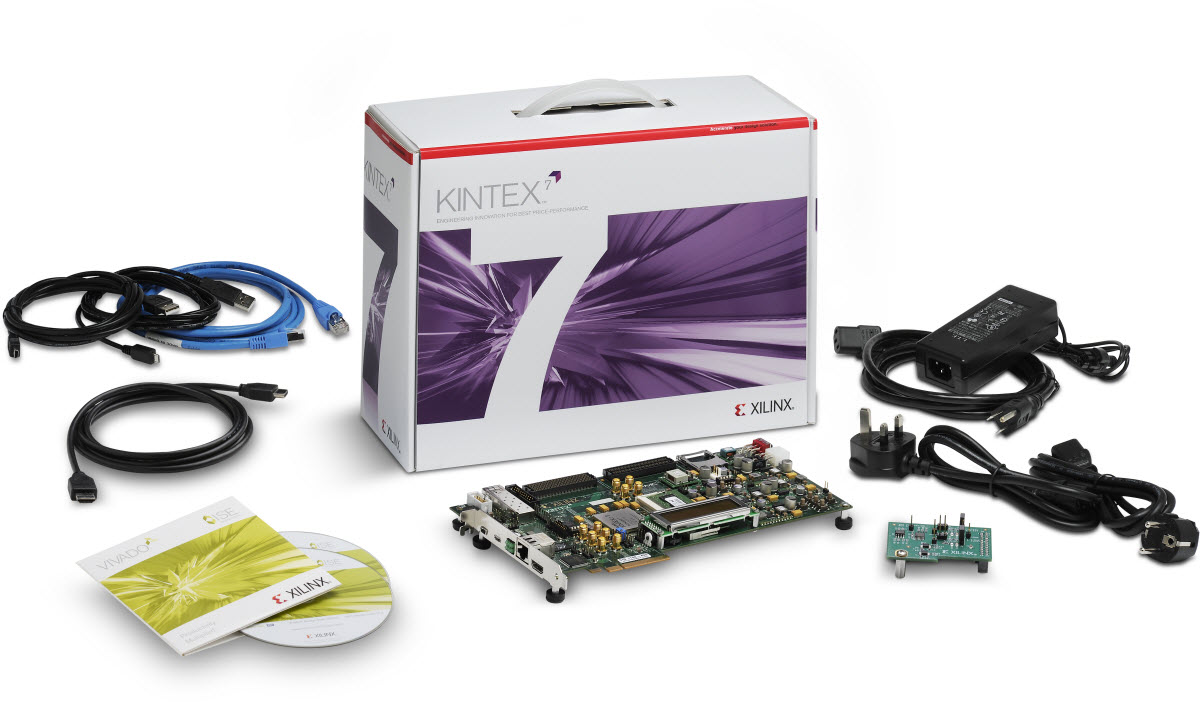
\includegraphics[width=0.7\textwidth]{fig/c3_desenvolvimento/intro/kintex-7_kc705}
\caption{Foto ilustrativa do kit de desenvolvimento Kintex-7 KC705 extraida do site da Xilinx.}
\label{fig:kc705}
\end{figure}

Para o desenvolvimento desse projeto, escolheu-se utilizar o kit de desenvolvimento da Xilinx\textregistered{} chamado Kintex-7 KC705.
O único critério utilizado foi a disponibilidade dos equipamentos no início do projeto e a capacidade do dispositivo de realizar a reconfiguração parcial dinâmica.
Este kit possui FPGA modelo XC7K325T-2FFG900C, leitor de cartão de memória, conector PCIe\textregistered{}, memória DDR3, visor de 7-segmentos e porta ethernet, dentre outros.

Escolheu-se ainda, de forma arbitrária, o uso da linguagem VHDL para a descrição de \textit{hardware} ao invés da Verilog.

\section{Experimentos}
Os experimentos desenvolvidos nos capítulos a seguir tem como objetivo o estudo da implementação da autorreconfiguração e todos os elementos que a acompanham.
Sendo assim, prova-se inicialmente que a reconfiguração é de fato dinâmica através de um experimento.
Em seguida, para suportar o requisito de memória da autorreconfiguração, estuda-se as memórias e desenvolve-se um experimento para colocar este conhecimento em prática.
Logo depois, espera-se entender a formação dos arquivos binários utilizados na reconfiguração e desenvolver um experimento que consiga interpretar algum cabeçalho existente.
Por último, a autorrenconfiguração se tornará o objetivo principal de um experimento visando entender as interfaces utilizadas para este fim. 

%%%%%%%%%%%%%%%%%%%%%%%%%%%%%%%%%%%
%					 Experimento 1
%%%%%%%%%%%%%%%%%%%%%%%%%%%%%%%%%%%

\chapter{Experimento 1 - Reconfiguração Dinâmica}
De forma a dar validade a todo o projeto, desenvolveu-se um experimento para entender o processo de desenvolvimento de sistemas reconfiguráveis dinamicamente e algumas peculiaridades do kit de desenvolvimento.
Este experimento tem como objetivo a construção de um projeto que se utilize de reconfiguração dinâmica para reprogramar um FPGA.

\section{Introdução Teórica}
Antes de se começar a construir o experimento, é necessário estudar as peculiaridades da placa e deste tipo de projeto, bem como seu fluxo de desenvolvimento.
Este estudo é apresetado a seguir.

\subsection{Peculiaridades}
O kit de desenvolvimento utilizada apresenta várias peculiaridades com relação aos kits comuns.
A única que afeta diretamente o experimento em questão é o uso de um relógio com sinal diferencial ao invés do sinal comum, explicado a seguir.
Outra peculiaridade é uma diferente estrutura de organização de arquivos, que permite um desenvolvimento mais limpo e de fácil entendimento.

\subsubsection{Relógio Diferencial}
Diferentemente das FPGAs comuns, a que está presente neste kit contém um relógio diferencial, ou seja, ele é composto por dois sinais ao invés de um.
A razão para tal é a presença de circuitos sensíveis a interferências, tais como \textit{transceivers}, que são muito menores em sinais diferenciais.
O kit disponibiliza duas opções de relógio: o SYSCLK e o USER\_CLOCK.
O primeiro possui uma frequência fixa de oscilação de 200 MHz.
O segundo possui uma frequência original de 156,250 MHz, mas pode ser programado através de uma interface I$^2$C para ter frequências entre 10 MHz e 810 MHz.
Nota-se porém que o uso do SYSCLK é bem mais simples que o do USER\_CLOCK, não sendo necessário nenhum circuito controlador/programador.

O Xilinx Design Tools disponibiliza uma ferramenta chamada \textit{CORE Generator} para a construção de diversos tipos de circuitos de propriedade intelectual.
Dentre eles se encontra o guia \textit{Clocking Wizard}, que pode construir elementos para transformar o sinal do relógio em um sinal simples.
Através dele também é possivel utilizar as PLLs da placa para modificar a frequência deste sinal para valores entre 20 MHz e 800 MHz.

\subsubsection{Estrutura de Pastas}
A questão da organização do projeto em pastas bem específicas foi bem reforçado na literatura \cite{ug702, ug743, ug744}.
Os manuais recomendam a estrutura de pastas apresentada abaixo.
\begin{lstlisting}
Projeto/
  Source/           //codigos-fonte organizados segundo particao
  Implementation/   //contem pastas para cada config. dinamica gerada
  Synth/            //contem pastas com os arquivos .xst e .prj
  Tools/            //ferramentas para automacao da sintese
  PlanAhead/        //pasta para o projeto do PlanAhead
\end{lstlisting}
A principal razão para esta recomendação é o uso de ferramentas variadas, tais como \textit{scripts} em TCL, o XST e o PlanAhead.
Esta estrutura de pastas foi obedecida por ajudar a manter o ambiente de desenvolvimento limpo.

\subsection{Fluxo de Ferramentas}
Uma das primeiras coisas que se destaca no desenvolvimento de dispositivos dinamicamente reconfiguráveis é a diferença no fluxo de ferramentas, também conhecido como \textit{software tools flow}, em relação ao fluxo tradicional \cite{ug743}.
Esta diferença é motivada pela necessidade de construção de diversos \textit{bitfiles} parciais, ao contrário de outros projetos, onde objetivo final é um arquivo binário completo.

Como pode-se ver da figura \ref{fig:ex1:softwareflow}, o fluxo tradicional requer apenas o uso do programa ISE, e opcionalmente do XPS e do SDK, para a construção de um projeto de \textit{hardware} e o iMPACT para a programação da FPGA.
No fluxo para reconfiguração dinâmica, porém, mostrado na figura \ref{fig:ex1:prsoftwareflow}, além das ferramentas do fluxo tradicional, faz-se necessário o uso da ferramenta XST para a síntese do \textit{netlist} dos comportamentos das partições reconfiguráveis e do PlanAhead para a definição de partições e configurações.
Note que estes fluxos não apresentam as únicas opções de fluxo de ferramentas, mas as que foram utilizadas neste projeto.

\begin{figure}[h]
	\centering
       	\begin{subfigure}[b]{\textwidth}
       		\centering
		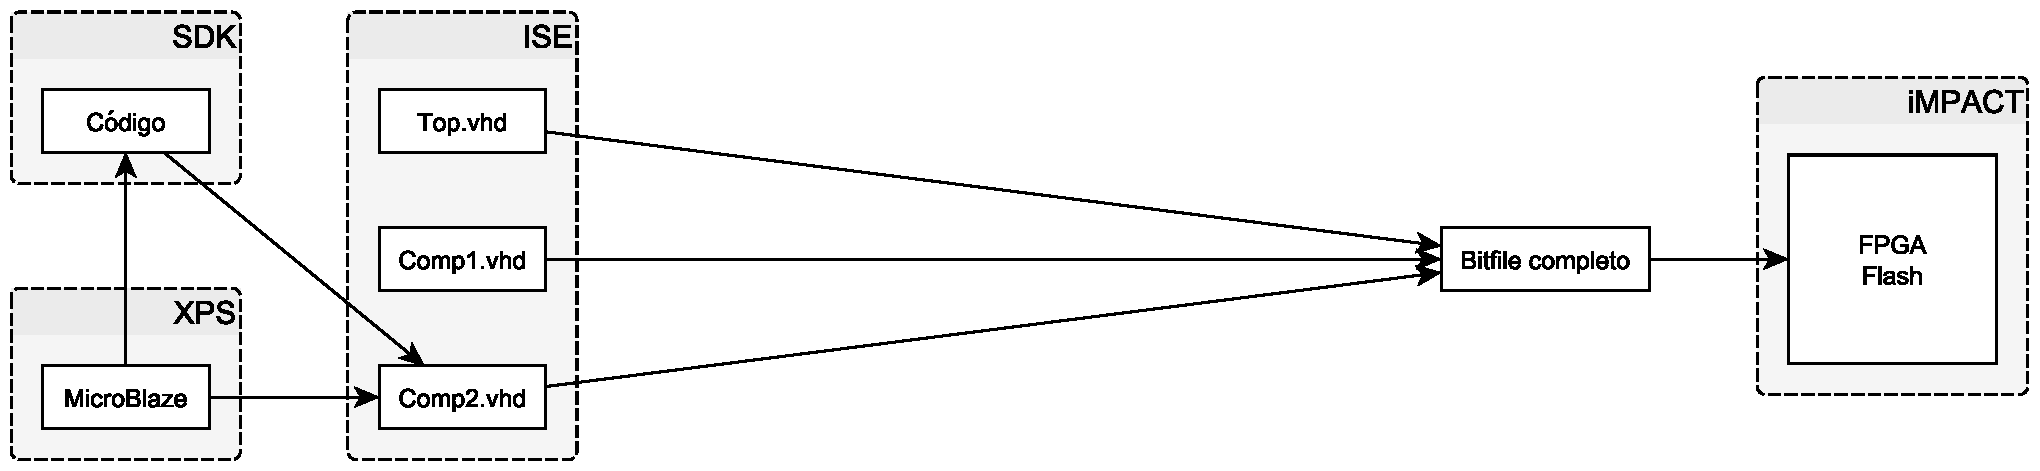
\includegraphics[height=100px]{fig/c3_desenvolvimento/ex1/softwareflow.pdf}
		\caption{Foto ilustrativa do fluxo de ferramentas tradicional. Note que o uso do microcontrolador MicroBlaze é opcional, tornando os primeiros blocos, SDK e XPS, também opcionais.}
		\label{fig:ex1:softwareflow}
	\end{subfigure}\\
	\begin{subfigure}[b]{\textwidth}
		\centering
		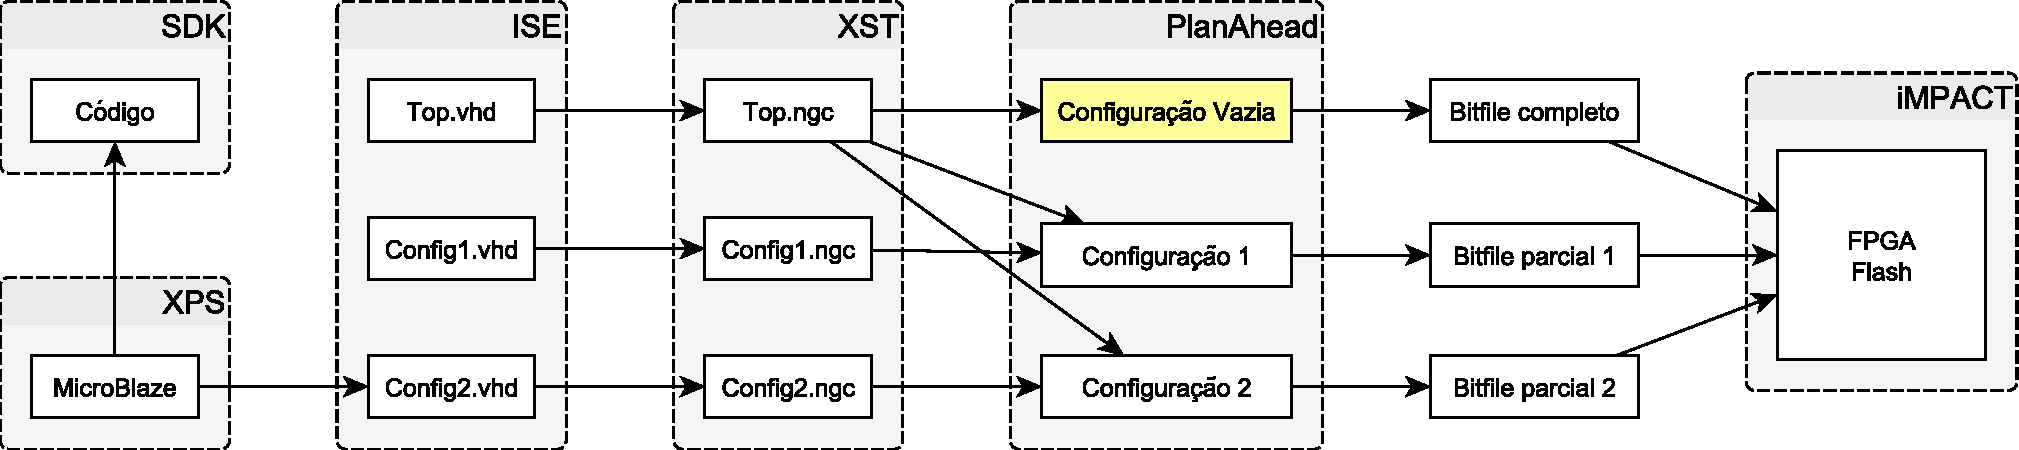
\includegraphics[height=100px]{fig/c3_desenvolvimento/ex1/prsoftwareflow.pdf}
		\caption{Foto ilustrativa do fluxo de ferramentas para a reconfiguração dinâmica. Assim como no caso tradicional, o uso do SDK e do XPS são opcionais. Note que o bloco em amarelo indica a configuração padrão, que será programada inicialmente. A escolha da configuração padrão é arbitrária.}
		\label{fig:ex1:prsoftwareflow}
	\end{subfigure}
	\caption{Comparação dos fluxos de ferramentas. Note que estes fluxos não apresentam as únicas opções de fluxo de ferramentas, mas as que foram utilizadas neste projeto.}
	\label{fig:ex1:softwareflow:comparacao}
\end{figure}

Note que a reconfiguração parcial pede uma síntese utilizando o método \qt{de baixo para cima} (\textit{bottom-up}), mas uma implementação \qt{de cima para baixo} (\textit{top-down}) \cite{ug743}, ou seja, a síntese acontece primeiro nos elementos de mais baixo nível, mas a implementação deve começar pelos de mais alto nível.
Isto acontece para que os requisitos de interfaceamento dos componentes reconfiguráveis sejam encontrados antes de se determinar como incluí-los no projeto, a partir de onde se continua o processo normal de implementação.
Note também que a implementação deve garantir que a lógica em comum, ou estática, seja implementada da mesma forma para as diferentes configurações \cite{ug702}.

\section{Experimento}
Para se entender mais a fundo o fluxo de projeto, nada melhor que construir um projeto.
Implementou-se para isto o sistema esquematizado na figura \ref{fig:ex1:componentes}.
Este sistema contém o \qti{Top} para interfaceamento com a FPGA, o \qti{Clock\_Station} e o \qti{Clocks} para tratamento do sinal de relógio, a \qti{Static}, que possui um lógica estática para demonstrar que a reconfiguração de uma partição não interfere com outra, e a \qti{Dynamic}, que possui a lógica a ser alterada dinâmicamente.
A interface \qti{Top} possui conexões com os LEDs e o SYSCLK do dispositivo FPGA, bem como conexões de entrada e saída com os componentes instanciados nela.
O componente \qti{Clock\_Station} recebe a entrada de relógio diferencial e retorna 3 sinais de relógios simples, um com 1 Hz, outro com 2 Hz e o último com 5 Hz.

\begin{figure}[h]
\centering
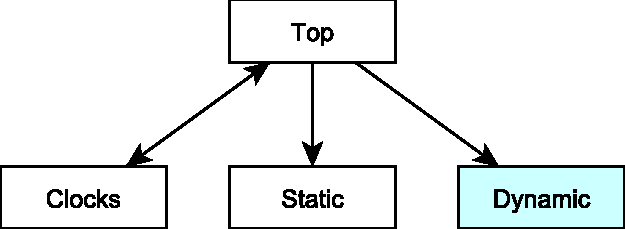
\includegraphics[width=0.5\textwidth]{fig/c3_desenvolvimento/ex1/componentes.pdf}
\caption{Foto ilustrativa do sistema desenvolvido para o teste de validação do experimento 1. Ele é composto por uma parte estática e uma parte dinâmica. O elementos em branco são estáticos, os em azul são dinâmicos e o em amarelo corresponde a um componente gerado automaticamente com o através das ferramentas da Xilinx.}
\label{fig:ex1:componentes}
\end{figure}

\subsection{Comportamento}
O projeto de um sistema parcialmente reconfigurável pode ser visto como vários projetos completos com partes em comum.
Seguindo essa lógica, dois projetos com comportamentos diferentes foram construídos usando como base a figura \ref{fig:ex1:componentes}.
O comportamento individual de cada módulo ou componente será descrito a seguir.
Este passo está ilustrado no fluxo de ferramentas da figura \ref{fig:ex1:prsoftwareflow} como ISE, visto que esta ferramenta da Xilinx é a mais utilizada para projetos comuns.

O componente \qti{Static} possui 3 entradas para relógios, um pulsando a 1 Hz, outro a 2 Hz e o teceiro a 5 Hz, e 3 saída paras LEDs.
Ele simplesmente liga as entradas (relógios) às saídas (LEDs), criando assim uma forma visual de comprovar que a reconfiguração do componente \qti{Dynamic} acontecerá dinamicamente.

O componente \qti{Dynamic} possui dois comportamentos distintos.
O primeiro deles é o de um simples contador crescente de 4 bits.
O segundo é uma máquina de estados que alterna os 4 bits de saída entre "1100" e "0011" a cada pulso de relógio.
Este componente possui uma entrada para um relógio pulsando a 1 Hz, que acionará as transições, e uma palavra de 4 bits de saída.
A frequência de operação deste componente foi escolhida para, junto com as frequências do \qti{Static}, permitir a visualação de que \qti{Static} não para de funcionar quando \qti{Dynamic} está sendo reconfigurado.

O componente \qti{Clocks} recebe os sinais diferenciais de relógio e o transformam em um sinal comum.
O bloco lógico utilizado para isso foi construído usando ferramentas presentes no ISE.
Uma vez que a ferramenta permitia a construção de um relógio com divisor de frequência, a frequência do relógio da placa, que nesse caso é de 200 MHz, foi reduzida para 20 MHz.

O módulo \qt{Top} instancia os componentes descritos acima e faz a interface dos mesmos com a FPGA.
O componente dinâmico precisa de uma declaração de protótipo para ser instanciado corretamente.
Utilizou-se o código abaixo para esta finalidade.
\begin{lstlisting}[style=customVHDL]
component dynamic
    port ( clk  : in  std_logic;
           leds : out std_logic_vector (3 downto 0));
end component;
\end{lstlisting}
O módulo \qt{Top} possui também um divisor de frequência para reduzir a frequência devolvida por \qt{Clocks} para 1 e 2 Hz.

\subsection{Síntese}
Com o comportamento do projeto definido, o próximo passo segundo o fluxo de ferramentas é a síntese, identificada no fluxo de ferramentas da figura \ref{fig:ex1:prsoftwareflow} como XST.
Este passo é necessário uma vez que o próximo passo, referente ao PlanAhead, não aceita como entrada códigos-fonte, mas arquivos conhecidos como \textit{netlists}.
Os códigos-fonte precisam passar por uma etapa de síntese separada para poderem ser importados no PlanAhead.

O comando XST (\textit{Xilinx Synthesis Tool}), responsável por realizar a síntese, recebe tipicamente um \textit{script} contendo o endereço dos códigos-fonte, o nome do arquivo de saída, o tipo do arquivo de saida, o modelo da FPGA utilizada e uma indicação do código-fonte principal.
O comando para iniciar o processo é o seguinte.
\begin{lstlisting}[style=customVHDL]
xst.exe -ifn Top.xst
\end{lstlisting}
O arquivo \qt{Top.xst} contém os seguintes comandos.
\begin{lstlisting}[style=customVHDL]
run
-ifn Top.prj
-ofn Top
-ofmt NGC
-p xc7k325t-2-ffg900
-top top
\end{lstlisting}
O arquivo \qt{Top.prj} contém os endereços dos arquivos, conforme a seguir.
\begin{lstlisting}[style=customVHDL]
vhdl work "../../Sources/static/top.vhd"
vhdl work "../../Sources/static/static.vhd"
vhdl work "../../Sources/static/clocks.vhd"
vhdl work "../../Sources/static/clock_station.vhd"
\end{lstlisting}\

Note que estes comandos e arquivos indicados acima são para síntese dos componentes estáticos.
Uma vez que não existe nenhuma restrição especial para tais componentes, eles podem ser síntetizados para um único arquivo de saída.
O mesmo não pode ser dito para os elementos dinâmicos.
Cada componente dinâmico precisa ser sintetizado em separado para depois ser incluído no projeto através do PlanAhead.

A síntese de componentes dinâmicos precisa ser realizada com um \textit{script} \qt{.xst} ligeiramente diferente.
Como mostrado a seguir, faz-se necessária a inclusão do argumento \qt{-iobuf NO}, que desabilita a inserção de componentes de Entrada/Saída \cite{ug743, ug748}.
\begin{lstlisting}[style=customVHDL]
run
-ifn DynFSM.prj
-ofn DynFSM
-ofmt NGC
-p xc7k325t-2-ffg900
-top dynamic
-iobuf NO
\end{lstlisting}
Note que o arquivo \qt{DynFSM.prj} contém informações sobre o código-fonte do componente dinâmico, como mostrado a seguir.
\begin{lstlisting}[style=customVHDL]
vhdl work "../../Sources/dynamic_fsm/dynamic.vhd"
\end{lstlisting}

Existe também a possibilidade de construção de um \textit{script} para a síntese automática de todos os arquivos.
Utilizou-se aqui uma adaptação do arquivo em linguagem TCL usado pela Xilinx em seus manuais e exemplos \cite{ug702, ug743, ug744}.
A única função deste \textit{script} é a construção dinâmica dos comandos com base em listas de arquivos pré-informados.

\subsection{PlanAhead}
Com os arquivos síntetisados, pode-se começar a etapa referente ao PlanAhead.
Nela, importa-se os arquivos da etapa anterior, cria-se a partição reconfigurável, mapea-se esta partição no dispositivo, cria-se configurações alternativas, promove-se tais configurações e gera-se os \textit{bitfiles} para a programação do dispositivo.
Note que é preciso uma licença do ISE que permita o uso do PlanAhead e de reconfiguração parcial para a realização desta etapa.

O primeiro passo necessário no PlanAhead é a criação do projeto.
Para isso, após a abertura do programa, clica-se no ícone superior esquerdo mostrado na figura \ref{fig:ex1:planahead}, onde se lê \qt{Create New Project}.
Na janela que aparece, indica-se o nome do projeto e seu caminho, lembrando que foi criada uma pasta anteriormente especificamente para conter este projeto.
Indica-se também que o projeto é do tipo \qti{Post-synthesis Project} e que deseja-se habilitar a reconfiguração parcial, indica-se quais \textit{netlists} compõe o comportamento estático do sistema e qual destes corresponde ao arquivo principal (\qti{Top}), qual é o arquivo de restrições (\textit{constrains}) e qual é o modelo da FPGA.

\begin{figure}[h]
\centering
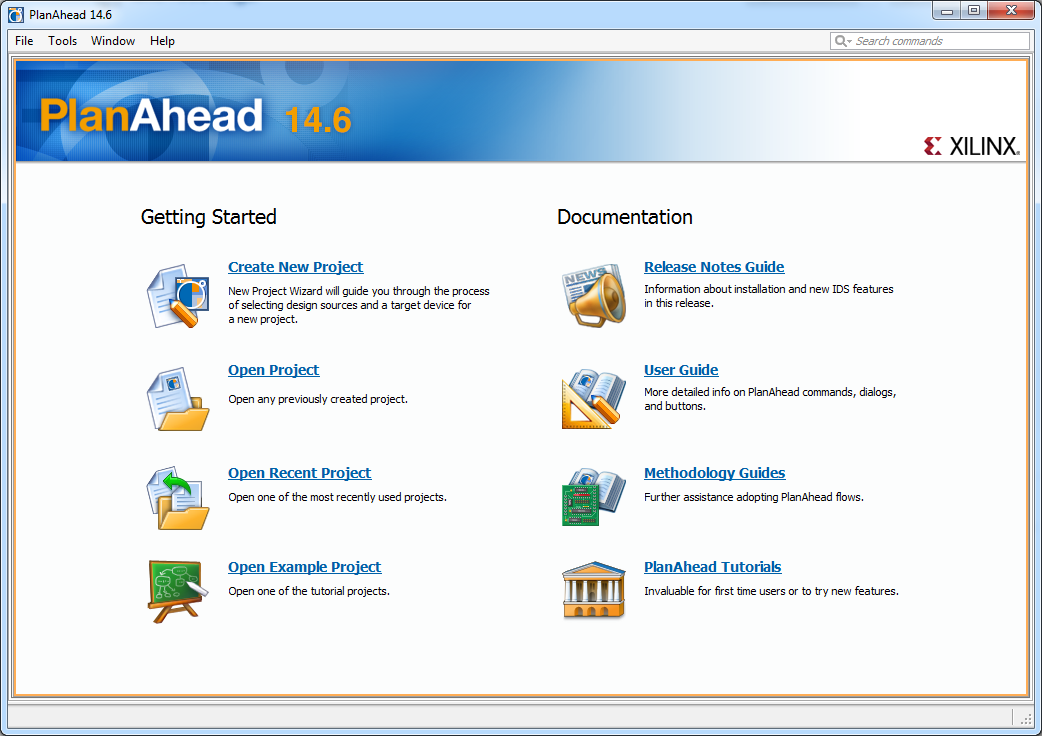
\includegraphics[width=0.9\textwidth]{fig/c3_desenvolvimento/ex1/PlanAhead}
\caption{Imagem do PlanAhead logo que aberto.}
\label{fig:ex1:planahead}
\end{figure}

Após a criação do projeto, carregam-se os arquivos sintetizados abrindo \qti{Open Synthesized Design}, presente no painel \qti{Flow Navigator} sob a opção \qti{Netlist Analysis}.
Duas janelas de avisos aparecem, informando que existe uma partição não implementada e aviso sobre alguns pinos.
Estes avisos podem ser desconsiderados.

Pode-se agora definir a partição que armazenará o componente dinâmico.
Isso é feito através do painel \qt{\textit{Netlist}}, selecionando-se a opção \qt{\textit{Set Partition}} do menu que aparece ao se clicar em \qt{dynamic\_i} com o botão direito.
Na janela que aparece, seleciona-se a opção referente à partição reconfigurável, nomea-se o módulo reconfigurável de acordo com o componente que será carregado e indica-se o arquivo (NGC) que corresponde ao arquivo sintetizado do componente reconfigurável.
Não é necessário informar restrições, visto que o componente, seguindo recomendações, não acessa os pinos de entrada e saída diretamente.
Note ainda que é recomendado que o primeiro módulo a ser incluído seja o mais complexo e sucetível a falhas, permitindo que erros e falhas na definição da região a seguir sejam identificados mais cedo.

Precisa-se definir também uma região para a partição recém criada.
Isto pode ser feito pelo mesmo painel \qti{Netlist}, selecionando-se a opção \qti{Set Pblock Size} do menu que aparece ao se clicar em \qt{dynamic\_i} com o botão direito.
Nesse momento, precisa-se selecionar na aba \qti{Device} uma região do dispositivo que contenha uma quantidade de recursos maior que a requerida pelo projeto.
Note que o processo de escolha dessa região não é bem definido, o que abre espaço para diversos erros de alocação.
Para testar se a região foi bem alocada, abre-se a aba \qti{Design Runs} do painel inferior, clica-se com o botão direito na única configuração disponível no momento e seleciona-se \qti{Run Launch}.
Este processo pode demorar.
Em tentativas subsequentes, seleciona-se a opção de recomeçar todo o processo do zero, evitando de se utilizar arquivos gerados em execução anteriores.
Uma região já testada e comprovada para este experimento é a que contém as células (\textit{slice}) de X80Y244 a X139Y205.
Ela pode ser selecionada na aba \qti{Device}, após se ampliar o mapa de recursos até que os nomes dos elementos lógicos, em cinza, fiquem visíveis.
Outra possibilidade, um pouco mais determinística, é descrita na seção \ref{par:alocacao}.

Ao final do \qti{Design Run} aparece uma janela que pergunta o que fazer em seguida.
Deve-se selecionar a opçao \qti{Promote Partitions} para exportar o resultado do mapeamento e roteamento da parte estática e informações da partição reconfigurável.
Estas informações serão utilizadas nos passos seguintes para construir configurações alternativas compatíveis com a primeira.
Na janela que se abre, deve-se marcar as configurações implementadas.

Após promover a primeira configuração, adiciona-se duas novas possibilidades de módulos reconfiguráveis para esta partição: um com comportamento definido e outro vazia.
Para isso, clica-se em \qti{Synthesized Design} novamente e seleciona-se a opção \qti{Add reconfigurable module} do menu que aparece ao se clicar em \qt{dynamic\_i} no painel \qti{Netlist} com o botão direito.
O processo é o mesmo da definição da partição, sendo a única mudança na seleção do arquivo sintetizado e do nome do módulo.
O módulo vazio pode ser criado usando esta mesma opção, mas selecionando-se a opção que indica a inclusão de uma \textit{black box} sem o uso de uma \textit{netlist}.

Com as possibilidades de módulos reconfiguráveis definidas, pode-se construir várias configurações.
Isso é feito através do clique com botão direito na \qti{Design Runs} do painel inferior e selecionando-se a opção \qti{Create Runs...}.
A janela que abre possui um painel chamado \qti{Create Implementation Runs}.
Nesse painel, na coluna \qti{Partition Action}, define-se, na coluna \qti{Module Variant} da nova janela que aparece, o módulo desejado.
Voltando para a primeira janela, clica-se em \qti{More} para adicionar a última configuração desejada.
Note que, quando definindo o \qti{Partition Action}, a linha referente a \qti{Static Logic} deve possuir \qti{Import} na coluna \qti{Action}, indicando que a parte estática não será implementada, mas sim importada de implementações anteriores.

Em seguida, uma janela aparece perguntando o que fazer com estas novas configurações.
Deve-se selecionar a opção \qti{Launch runs on local host} para iniciar suas implementações.
Este processo é demorado, mas mais rápido que o da primeira configuração.
Note que os avisos que aparecerem podem ser ignorados.

Também é necessário promover estas novas configurações.
No menu de quando se clica com o botão direito sobre as configurações já existentes do painel \qti{{Configurations}}, seleciona-se \qti{{Promote Configuration...}}.
A promoção de uma configuração é o equivalente a sua exportação \cite{ug748}.
Promover a primeira configuração antes de implementar novas contribui para manter a parte estática, compartilhada, igual em todas as configurações, uma vez que elas não mais são sintetizadas e sim importadas.

Recomenda-se ainda fazer a verificação das configurações através do painel \qti{{Configurations}}.
Clicando-se com o botão direito, encontra-se a opção \qti{{Verify Configuration...}}, que faz com que uma janela seja aberta.
Selecionado-se todos os itens e clicando em \qti{{OK}}, a verificação se inicia.
Nenhum erro deve ser encontrado.

O último passo necessário para a criação dos \textit{bitfiles} é o \qti{{Generate Bitstream}}, localizado no menu a esquerda.
Este passo recebe o resultado das sínteses e implementações e transforma-os em \textit{bitfiles}.
Ele precisa ser realizado com todas as configurações do \qti{Design Runs} selecionados ou alguma delas não terá seus arquivos binários gerados.
Após o termino deste processo, os tais \textit{bitfiles} podem ser encontrados na pasta do projeto, dentro das pastas com nome de cada configuração que ficam dentro de da pasta \qt{*.runs}.
Existem dois arquivos \textit{.bit} dentro de cada pasta, um maior, que contém a configuração completa, e outro menor, que possui a configuração parcial.

\subsection{iMPACT}
Com os \textit{bitfiles} em mãos, usa-se-os para programar a FPGA através da ferramenta iMPACT. 
A primeira coisa a se fazer após abrir o programa é permitir que o sistema crie um projeto automaticamente.
Na janela que se abre, escolhe-se a opção \qt{\textit{Automatically connect to a cable and identify Boundary-Scan chain}} do item \qt{\textit{Configure devices using Boundary-Scan (JTAG)}}.
Quando pergunta-se se deseja-se atribuir uma nova configuração, pode-se clicar que sim e escolher um arquivo binário completo gerado na etapa anterior.
Normalmente escolhe-se a configuração vazia como configuração inicial para poupar energia.

Quando a configuração for completamente transmitida e implementada, observa-se que um LED está piscando com uma frequência de 2 Hz e todos os outros (acionados) estão acesos.
Isto acontece uma vez que o sitema atribui sinal ativo para os elementos desconectados.

Para realizar a reconfiguração parcial dinâmica, clica-se com o botão direito no símbolo do dispositivo que aparece no iMPACT e seleciona-se a opção \qt{\textit{Assign New Configuration File...}}.
Procura-se então pelos arquivos binários parciais localizados na pasta \textit{PlanAhead > PlanAhead.runs >} \qt{nome da configuração}.
Este arquivo possui \qt{partial} em seu nome, o que o diferencia do arquivo binário completo.
Note que utilizar os arquivos binários completos não gera erro, mas constitui reconfiguração total, não parcial.
Após a seleção da configuração desejada, o último passo necessário é a programação, que pode ser realizada clicando-se com o botão direito no dispositivo e selecionando-se a opção \qt{\textit{Program}}.

\subsection{Possíveis Erros}
Esta seção é destinada apenas para a solução de alguns erros encontrados durante a realização deste experimento.
É muito provável que, se o experimento for desenvolvido exatamente como mostrado aqui, nenhum destes erros aconteça.

\subsubsection{Erros no código-fonte} Este é um dos erros mais comuns.
A melhor forma de previní-lo é através da construção dos diversos comportamentos/configurações individuais utilizando o ISE.
Para acelerar o processo, realiza-se apenas a síntese.
Outra possibilidade é o uso do XST diretamente \, reduzindo ainda mais o tempo desta verificação. 

\subsubsection{Erro no carregamento do módulo reconfigurável}
Este erro, do PlanAhead, em geral acontece quando o componente instanciado no \qti{Top} possuem sinais diferentes do instanciado no \qti{Dynamic}.
Para corrigí-lo, deve-se verificar os códigos-fonte, síntetizá-los novamente, limpar a pasta \qt{PlanAhead} e recomeçar este passo (PlanAhead) novamente.

\subsubsection{Erros na alocação de partições}
\label{par:alocacao}
Um erro bastante comum que aparece no PlanAhead é o de erro de alocação\footnote{\textit{AR\# 53290: Partial Reconfiguration - 7 series device layout of tiles (CLB, DSP, BRAM, INT) and a shared clocking structure of vertical clock spines between interconnect (routing) tiles}. Disponível em \url{http://www.xilinx.com/support/answers/53290.htm}}.
Existem duas possíveis formas de corrigí-lo: modificando-se o arquivo de restrições (UCF) ou alterando a região da partição.
A primeira forma, que ajuda a garantir que todos os recursos reconfiguráveis estão incluidas na região da partição, é a inclusão de \qt{INCLUSIVE=ROUTE} na linha que contém \qt{INST "dynamic\_i" AREA\_GROUP = "pblock\_dynamic\_i"}.

A segunda forma é simplemente mudando a posição da região da partição para a direita, para a esquerda ou sua largura, de acordo com a mensagem de erro retornada.
Esta método não é determinístico e pode ser necessárias várias tentativas antes de se conseguir uma partição mapeável. 
Este processo pode também ser realizado através do arquivo de restrições (UCF).
O código abaixo contém uma alocação de partição funcional para este experimento, podendo ser copiada sobre a definição atualmente existente no arquivo UCF.
\begin{lstlisting}
INST "dynamic_i" AREA_GROUP = "pblock_dynamic_i";
AREA_GROUP "pblock_dynamic_i" RANGE=SLICE_X80Y205:SLICE_X139Y244;
AREA_GROUP "pblock_dynamic_i" RANGE=DSP48_X3Y82:DSP48_X5Y97;
AREA_GROUP "pblock_dynamic_i" RANGE=RAMB18_X3Y82:RAMB18_X5Y97;
AREA_GROUP "pblock_dynamic_i" RANGE=RAMB36_X3Y41:RAMB36_X5Y48;
\end{lstlisting}

O arquivo UCF pode ser aberto pelo painel \qti{Sources} sob a árvore \qti{Constrains}.
Em caso de mais de um arquivo UCF presente, o desejado pode ser identificado pela marcação \qti{(target)} ao lado.
Dois cliques são suficientes para abrí-lo. 

\subsubsection{Esquecer de promover a partição}
A promoção da primeira configuração antes de se implementar as seguintes contribui para a implementação de configurações compatíveis.
Esquecer de promover esta partição pode fazer com que erros sejam gerados na etapa de verificação das partições.

\subsubsection{O PlanAhead pode travar enquanto implementando uma configuração}
Apesar de mais raro, o PlanAhead pode travar quando implementando uma configuração.
A melhor solução é o reinício do computador, visto que o programa bloqueia alguns arquivos durante a implementação e não os desbloqueia quando fechado forçadamente.

\subsubsection{Erros na detecção da placa}
Note que algum programa aberto pode interferir com a varredura realizada pelo iMPACT, fazendo-a falhar.
Para prevenir este erro, deve-se fechar o XPS, o SDK e qualquer outro programa que possa se utilizar das interfaces USB.
Note ainda que a placa deve estar ligada para poder ser detectada.

\subsubsection{Erro na geração do arquivo binário}
Na geração do arquivo binário, o erro BitGen:342 pode aparecer \footnote{\qti{AR\# 51813
14.2 BitGen - "ERROR:Bitgen:342 occurs after adding probes to the design in the case of 7 series devices"}, \url{http://www.xilinx.com/support/answers/51813.html}}.
Este erro aparece devido ao uso de pinos não explicitados no arquivo UCF, fazendo com que o PlanAhead tenha que usar as configurações padrões nestes pinos.
Uma forma de solucionar este problema é acrescentando a opção \qt{-g UnconstrainedPins:Allow} no comando do BitGen. 

\section{Resultados}
\subsection{Síntese}
A síntese ocorreu como esperado, gerando os arquivos sintetisados (NGC).
A figura \ref{fig:ex1:sintese} mostra o resultado do processo de síntese utilizando o \textit{script} Tcl.
\begin{figure}[h]
\centering
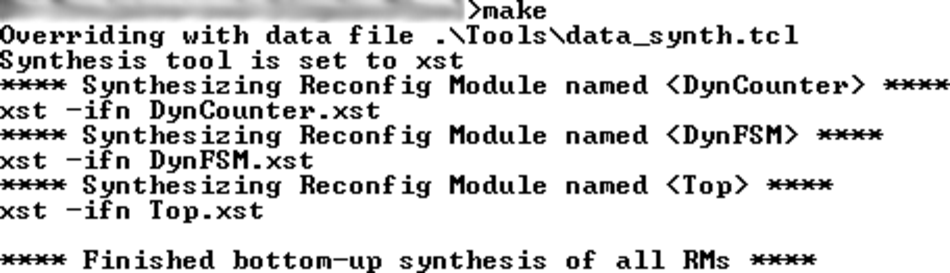
\includegraphics[width=0.6\textwidth]{fig/c3_desenvolvimento/ex1/Sintese.pdf}
\caption{Resultado da síntese.}
\label{fig:ex1:sintese}
\end{figure}

\subsection{PlanAhead}
O passo do PlanAhead foi bem sucedido, tendo gerado os arquivos binários como esperado.
O relatório de utilização do sistema, copiado abaixo, mostra que aproximadamente 1\% dos recursos do dispositivo foi utilizado.
\begin{lstlisting}
Slice Logic Utilization:
  Number of Slice Registers:                 2,734 out of 407,600    1%
    Number used as Flip Flops:               2,696
    Number used as Latches:                      3
    Number used as Latch-thrus:                  0
    Number used as AND/OR logics:               35
  Number of Slice LUTs:                      3,020 out of 203,800    1%
    Number used as logic:                    2,572 out of 203,800    1%
      Number using O6 output only:           1,962
      Number using O5 output only:             114
      Number using O5 and O6:                  496
      Number used as ROM:                        0
    Number used as Memory:                     338 out of  64,000    1%
      Number used as Dual Port RAM:            160
        Number using O6 output only:            96
        Number using O5 output only:             0
        Number using O5 and O6:                 64
      Number used as Single Port RAM:            0
      Number used as Shift Register:           178
        Number using O6 output only:           176
        Number using O5 output only:             1
        Number using O5 and O6:                  1
    Number used exclusively as route-thrus:    110
      Number with same-slice register load:    103
      Number with same-slice carry load:         6
      Number with other load:                    1
\end{lstlisting}

Note porém que a quantidade de elementos lógicos ocupados é maior devido ao roteamento.
O relatório que mostra este fenônemo foi copiado abaixo.
\begin{lstlisting}
Slice Logic Distribution:
  Number of occupied Slices:                 1,445 out of  50,950    2%
  Number of LUT Flip Flop pairs used:        3,851
    Number with an unused Flip Flop:         1,360 out of   3,851   35%
    Number with an unused LUT:                 831 out of   3,851   21%
    Number of fully used LUT-FF pairs:       1,660 out of   3,851   43%
    Number of slice register sites lost
      to control set restrictions:               0 out of 407,600    0%
\end{lstlisting}

A parte estática do dispositivo foi alocada como mostrado na figura \ref{fig:ex1:device}.
\begin{figure}[h]
\centering
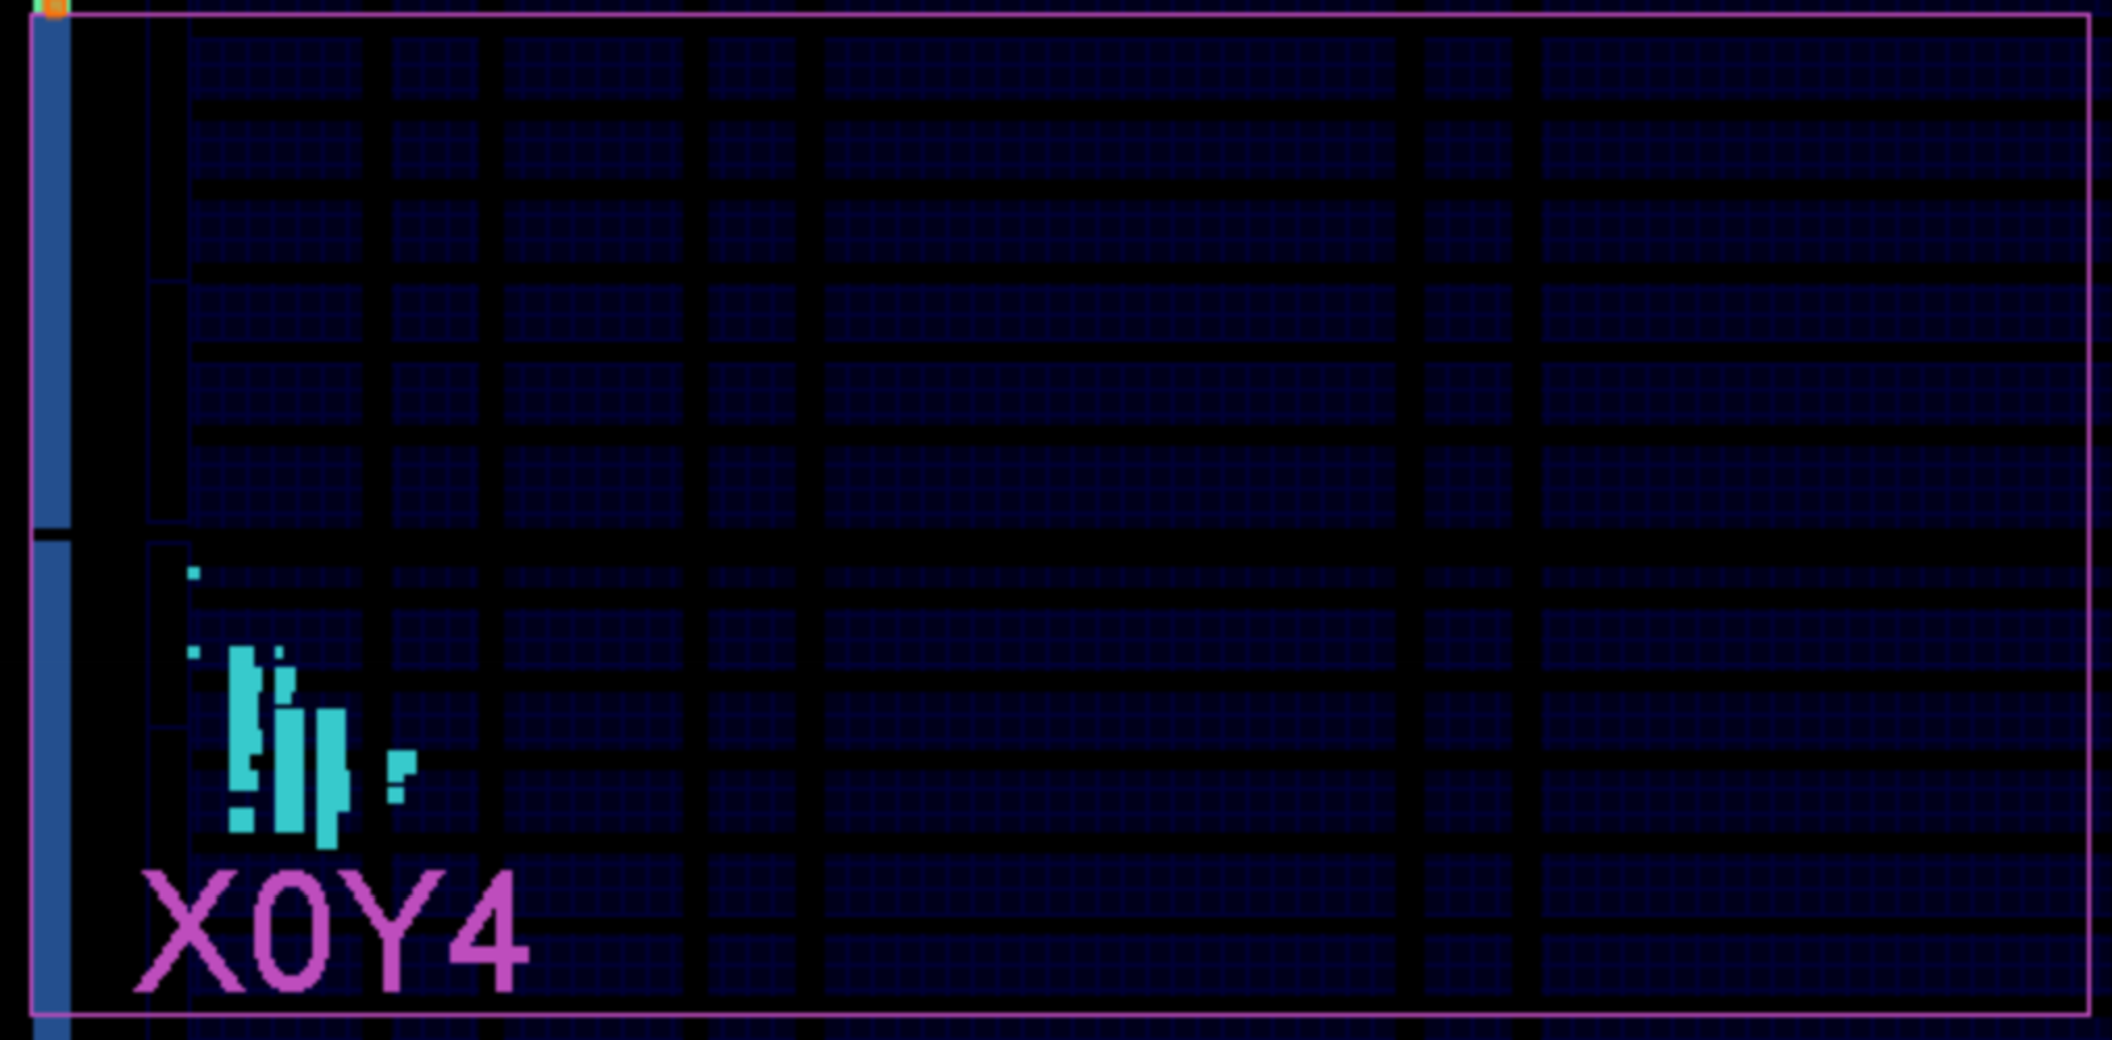
\includegraphics[width=0.7\textwidth]{fig/c3_desenvolvimento/ex1/Device.pdf}
\caption{Alocação da parte estática do projeto no dispositivo. Em azul claro estão os elementos lógicos utilizados.}
\label{fig:ex1:device}
\end{figure}

\subsection{iMPACT}
A etapa do iMPACT também foi bem sucedida.
A programação da configuração completa levou 10 segundos e a programação da configuração parcial levou 1 segundo.

\section{Conclusão}
O processo de desenvolvimento de partições reconfiguráveis e sua programação foi explorado e compreendido com sucesso.
Observou-se os pontos críticos do desenvolvimento e o fluxo mais adequado para a construção deste tipo de projeto, bem como alguns erros comuns e suas soluções.

%%%%%%%%%%%%%%%%%%%%%%%%%%%%%%%%%%%
%					 Experimento 2
%%%%%%%%%%%%%%%%%%%%%%%%%%%%%%%%%%%

\chapter{Experimento 2 - Memórias}
Seguindo o raciocínio apresentado no capítulo \ref{cap:introducao}, o próximo passo natural no desenvolvimento deste projeto é o entendimento do funcionamento das memórias.
Esta etapa abre caminho para que se armazene os arquivos binários de configurações parciais em uma memória embarcada, removendo a necessidade do computador para tal.

\section{Introdução Teórica}
Para o desenvolvimento deste experimento, faz-se necessário o estudo dos diferentes tipos de memórias, citando seus pontos fracos e fortes.
Também é necessário o estudo do MicroBlaze e das ferramentas XPS e SDK, visto que a forma mais direta de se trabalhar com memória em FPGAs é através do uso de microcontroladores embarcados.

\subsection{Tipos de Mémoria}
No kit utilizado existem vários tipos de memórias que poderiam ser usados, cada um com suas peculiaridades \cite{ug810}.
Este experimento foi dedicado à compreenção do funcionamento dos diversos tipos de memórias e à escolha da solução mais adequada.

\subsubsection{Memória \textit{Block RAM}}
A memória do tipo \textit{Block RAM} é construída usando-se os blocos de memória RAM restantes da FPGA.
Esta memória consegue alcançar velocidades de leitura na ordem de várias centenas de hertz, mas possui uma capacidade de armazenamento bem reduzida, de apenas 445 blocos de 36 Kb para este kit, totalizando um máximo de aproximadamente 2 MB \cite{ug473, wp377}.
Note que a configuração total da FPGA necessita de aproximadamente 11 MB, ou exatamente 91.548.896 bits, para sua programação total \cite{ug470}.
Pode-se programá-la através do iMPACT, dentre outras formas \footnote{\textit{Memory Initialization Methods}, escrito por Jim Wu em 31 de dezembro de 2011. Dísponível em \url{http://myfpgablog.blogspot.com.br/2011/12/memory-initialization-methods.html}}.

\subsubsection{Memória \textit{Distributed RAM}}
A memória \textit{Distributed RAM} é construida utilizando-se das LUTs disponíveis nas célula lógicas \cite{ug473, wp377}.
Também são muito rápidas, apesar de síncronas, e também possuem pouca capacidade de armazenamento.
Pode-se programá-la através do iMPACT, dentre outras formas.

\subsubsection{Memória \textit{Linear BPI Flash}}
A memória \textit{Linear BPI Flash} disponibiliza 128 Mb de memória não-volátil \cite{ug810}, acessadas em palavras de 16 bits.
Apesar disso, sua velocidade de leitura máxima é de 33 MHz.
Convertendo tal velocidade para a leitura de 32 bits, tem-se uma velocidade de leitura de aproximadamente 16 MHz.
Pode-se programá-la através do iMPACT.

\subsubsection{Memória \textit{SPI Flash}}
A memória SPI Flash é diferente na sua forma de acesso, que acontece através da interface SPI.
Esta memória fornece 128 Mb de memória não volátil \cite{ug810}.
Ela aceita três modos de operação, x1, x2 e x4, que corresponde a largura da palavra lida/escrita a cada pulso de relógio \cite{N25Q128}.
A frequência de operação é de no máximo 50 MHz \cite{xapp586}.
Pode-se programá-la através do iMPACT.

\subsubsection{Cartão de Memória SD}
O cartão de memória SD dá acesso a uma memória não-volátil de tamanho arbitrário.
Esta interface permite o uso de cartões de alto desempenho, lendo palavras de 4 bits a frequências de até 50 MHz \cite{ug810}.
A limitação desta interface é a dificuldade de leitura e escrita devido ao sistema de arquivos inerente ao cartão.
Note que também não existe a possibilidade de programação do cartão através do iMPACT, o que resolveria o problema do sistema de arquivos.

\subsubsection{\textit{CompactFlash} e o \textit{System ACE}}
\textit{System ACE} é um sistema que permite a programação de FPGAs e memórias voláteis a partir de um cartão \textit{CompactFlash} \cite{ds080, ds583}.
Este é bem robusto e popular em séries que possuem um leitor deste tipo de cartão, o que não é o caso desta.

\subsubsection{Memória DDR3}
A memória DDR3 é uma memória volátil com 1 GB de capacidade de armazenamento e possui uma frequência de operação da ordem dos 800 MHz \cite{MT8JTF12864HZ}.
Só pode ser programada apenas em tempo de execução, fazendo-se necessário o uso de um \textit{bootloader}.
Ela possui restrições de temporização extremamente apertadas e necessita do uso de componentes bastante escassos no FPGA.

\subsection{Fluxo de Projeto}
O procedimento para a construção de um projeto com MicroBlaze segue o fluxo descrito na figura \ref{fig:ex1:softwareflow}.
A figura \ref{fig:ex2:softwareflow} apresenta o fluxo de ferramentas para este caso específico.
Em outras palavras, o fluxo espera que primeiro se desenvolva o microprocessador com todos os seus periféricos para depois se desenvolver o programa que será embarcado.
Tanto o programa quando o processador gerarão arquivos binários que serão carregados pelo iMPACT através do SDK.

\begin{figure}[htp]
\centering
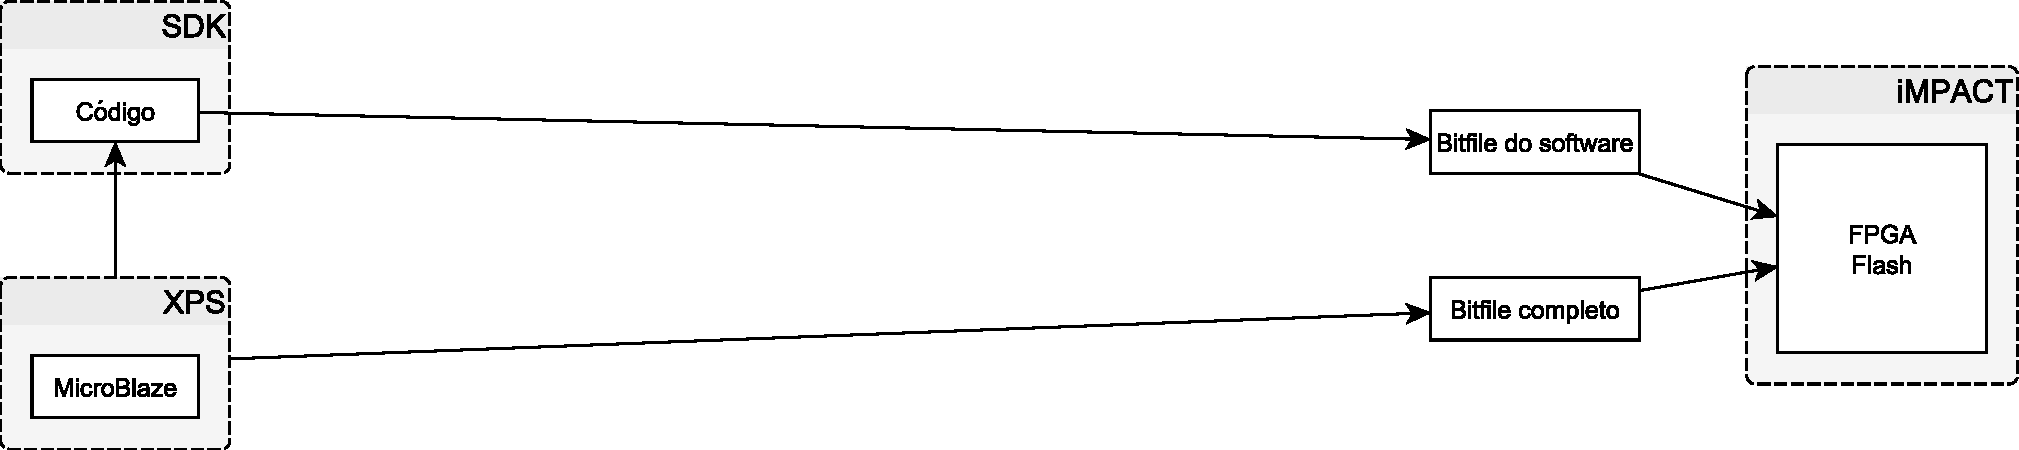
\includegraphics[height=100px]{fig/c3_desenvolvimento/ex2/softwareflow.pdf}
\caption{Foto ilustrativa do fluxo de ferramentas para o desenvolvimento de sistemas com MicroBlaze, extraído de \cite{ug081}.}
\label{fig:ex2:softwareflow}
\end{figure}

\subsection{MicroBlaze}
O MicroBlaze é um microprocessador otimizado para implementação em FPGAs da Xilinx \cite{ug081}.
Ele possui 32 registradores genéricos de 32 bits, instruções de 32 bits e endereços de 32 bits.
Seu \textit{pipeline} possui 3 ou 5 estágios e é construido em torno da arquitetura Harvard, como pode ser observado na figura \ref{fig:ex3:microblazecore}.
Todas as outras configurações, tais como o uso de \textit{Big Endian} ou \textit{Little Endian}, por exemplo, são opcionais \cite{ug081}.

\begin{figure}[h]
\centering
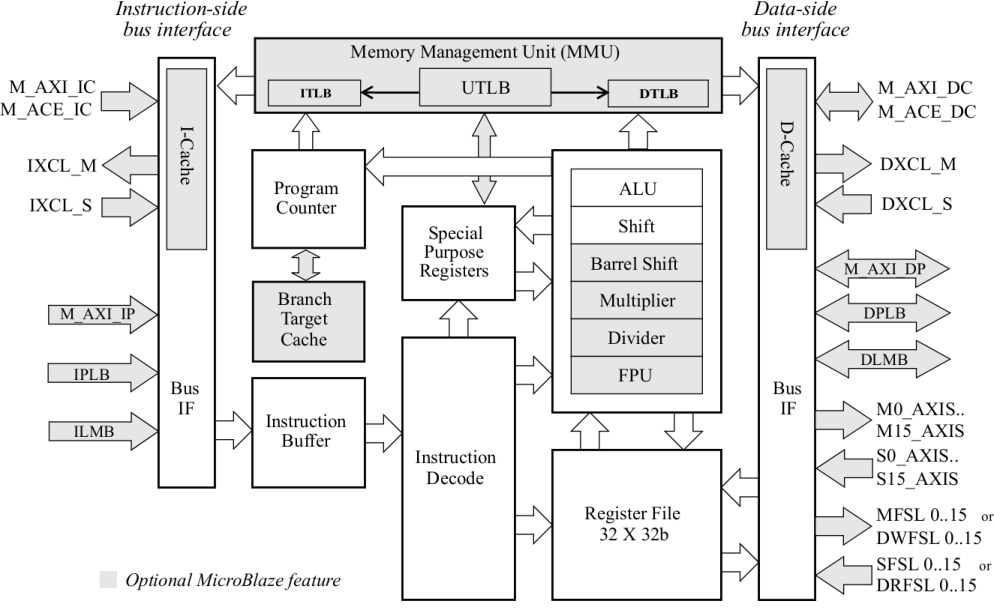
\includegraphics[width=0.75\textwidth]{fig/c3_desenvolvimento/ex2/MicroBlaze_Core.pdf}
\caption{Diagrama de blocos do MicroBlaze.}
\label{fig:ex3:microblazecore}
\end{figure}

O MicroBlaze permite o uso de diversas interfaces para comunicação com seus diversos periféricos, dentre elas a PLB, a LMB, a AXI e a ACE \cite{ug081}.
A interface mais atual suportada, e que foi utilizada neste experimento, é a Advanced eXtensible Interface 4 (AXI4) \cite{ug081, ug761}.
A AXI4 é uma interface mapeada em memória que oferece produtividade, flexibilidade e disponibilidade.
Ela possui três tipos de interfaces, a AXI4, a AXI4-Lite e a AXI4-Stream, onde as duas primeiras são compostam de 5 canais de comunicação: de leitura de endereço, de escrita de endereço, de leitura de dados, de escrita de dados e de escrita de resposta.

\section{Experimento}
Este experimento tem por objetivo o desenvolvimento de um sistema que instancie e acesse memórias capazes de armazenar as configurações parciais geradas no experimento anterior.
Para isto, deve-se entender o processo de construção de um processador embarcado MicroBlaze, com periféricos para acesso às memórias, e de construção de programa embarcado.
Deve-se ainda, antes de qualquer coisa, definir que tipo de memória é a mais apropriada para o objetivo traçado.

\subsection{Escolha da Memória}
Nota-se do primeiro experimento que os \textit{bitfiles} parciais gerados possuiam 645 KB cada, totalizando 1935 KB, ou 1,89 MB.
Com isso o uso das memórias que se utilizam de recursos internos da FPGA fica comprometido.
Observa-se também que a interface de reprogramação dinâmica, ICAPE2, utilizada em experimentos mais a frente, opera a uma frequência de até 100 MHz e pode receber palavras de até 32 bits, ou seja, 3200 Mb/s \cite{ug702}.
Por causa disso, todas as interfaces não-voláteis disponíveis acabariam se tornando gargalos no tempo de programação.

A única memória com tamanho e velocidade suficientemente grandes para este projeto é a memória DDR3.
Apesar disto, esta memória é volátil, necessitando ser inicializada sempre que o sistema é ligado.
Uma solução para este problema é a implementação de um sistema que carregue as informações de uma memória não-volátil, tanto a Linear Flash quanto a SPI Flash seriam suficientes, para a memória DDR3 em um momento inicial, e depois permita que a memória DDR3 seja acessada para a reconfiguração dinâmica, ou seja, através do uso de um \textit{bootloader}.

Sendo assim, optou-se por utilizar a memória QSPI Flash para uso na inicialização e a memória DDR3 para uso na execução.

\subsection{XPS}
Para começar, deve-se abrir o programa e criar um novo projeto usando o \textit{Base System Builder} (BSB), opção que corresponde ao item superior esquerdo do menu da tela inicial.
Na janela que aparece, escolheu-se a placa de desenvolvimento Kintex-7 KC705 \textit{Evaluation Platform}, \textit{Board Revision} C, e a opção de um só processador no sistema, para simplificar o projeto.
Dando prosseguimento, escolheu-se os periféricos desejados segundo a figura \ref{fig:ex2:bsb_prerifericos} e o tamanho das memórias local, de intrução e de dados, quiça, 128 KB, 8 KB e 8 KB respectivamente.
Modificou-se ainda, como pode-se ver na figura \ref{fig:ex2:bsb_prerifericos}, o \textit{Baud Rate} da interface UART para 115200 bits/s e o C\_SPI\_MODE da QSPI\_FLASH para \qti{Quad SPI Mode}.

\begin{figure}[htp]
\centering
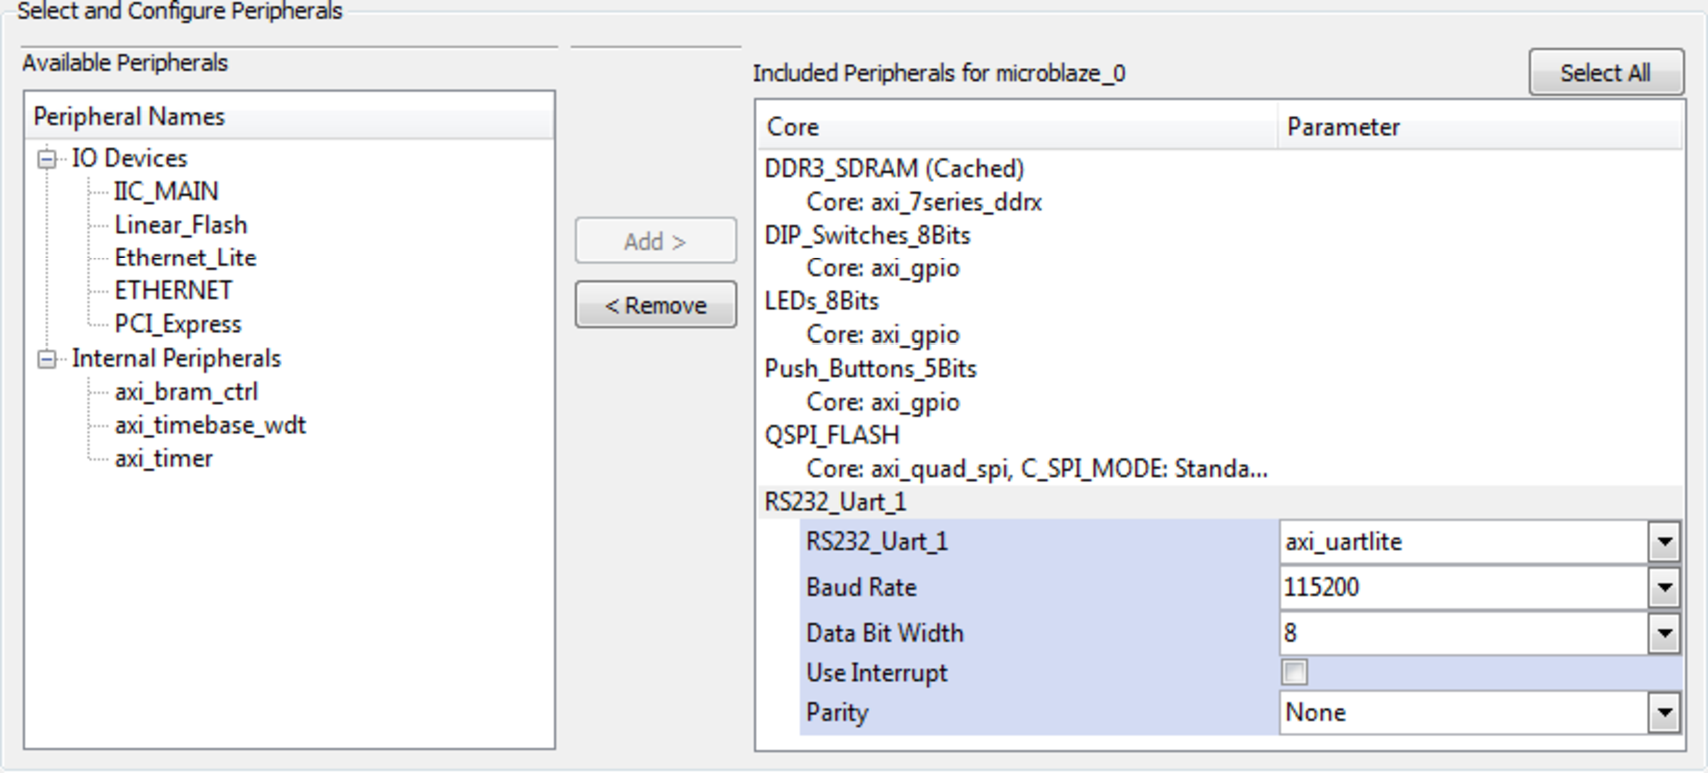
\includegraphics[width=0.9\textwidth]{fig/c3_desenvolvimento/ex2/BSB_AXI_flow.pdf}
\caption{Escolha dos periféricos no BSB do XPS.}
\label{fig:ex2:bsb_prerifericos}
\end{figure}

Antes de concluir o a construção do sistema, precisa-se ajustar os tamanhos das memórias e seus endereços, de forma que estes novos tamanhos possam ser corretamente acessados.
Isto pode ser feito na aba \textit{Addresses} do painel \textit{System Assembly View}.
Muda-se então o tamanho da memória SPI Flash para 128M, seu endereço base para 0x80000000, o tamanho da memória DDR3 para 1G e seu endereço base para 0xC0000000, conforme a figura \ref{fig:ex2:xps_enderecos}.
Note que o endereço-base da memória SPI Flash tem como única restrição de os 28 bits menos significativos iguais a zero e que o endereço-base da memória DDR3 tem esta mesma restrição para os 30 bits menos significativos.
Estas restrições são devido aos tamanhos das memórias e o alinhamento dos espaços de dados na memória.

\begin{figure}[htp]
\centering
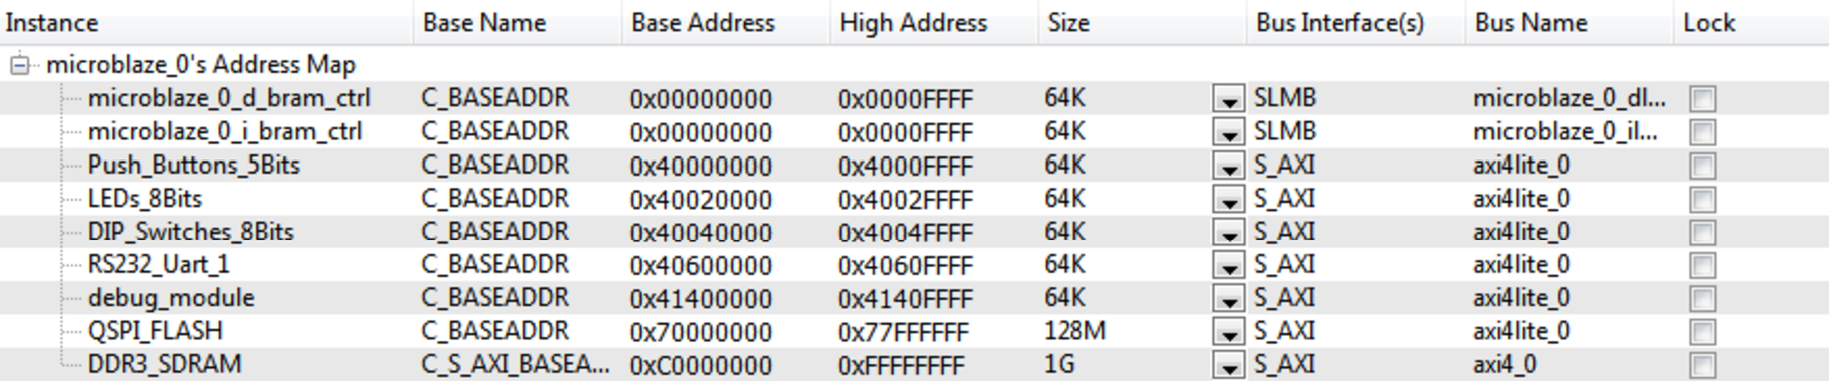
\includegraphics[width=0.8\textwidth]{fig/c3_desenvolvimento/ex2/xps_address.pdf}
\caption{Aba \textit{Addresses} do \textit{System Assembly View} indicando os ajustes dos endereços e tamanhos das memórias.}
\label{fig:ex2:xps_enderecos}
\end{figure}

Precisa-se ainda modificar as posições de memória cobertas pela memória \textit{cache}.
Isto é feito clicando-se duas vezes sobre \qt{microblaze\_0} na aba \qt{\textit{Bus Interfaces}} do painel \qt{\textit{System Assembly View}}.
Na janela que se abre, clica-se  \qt{\textit{Next}} 3 vezes para chegar página sobre \textit{caches}.
Modifique os endereços nas duas colunas para 0xc0000000 e 0xffffffff, indicando que a memória de instruções e memória de dados podem acessar os endereços da memória DDR3.
Apenas os endereços contidos neste intervalo da memória de dados podem ser escritos.
Note que o sistema reserva para uso próprio os primeiros 64K endereços das memórias, que correspondem às posições com finais entre 0x0000 a 0x3fff.
A tentativa de uso destes endereços comprometerá o correto funcionamento do sistema.

Algumas outras configurações também podem ser ajustadas, mas não sao estritamente necessárias para este experimento.

O projeto pode ser sintetizado através do botão \qt{\textit{Generate Netlist}} localizado no menu a esquerda e no menu \qt{\textit{Hardware}} da barra de menus.
Este processo é demorado.
Quando terminado, pode-se exportar o projeto através do botão \qt{\textit{Export Design}} para abrir o SDK com as informações deste processador.
Na janela que aparecer, marque \qt{\textit{Include bitstream and BMM file}} e clique em \qt{\textit{Export \& Launch SDK}}.
O arquivo binário contém informações da configuração da FPGA enquanto o arquivo BMM apresenta um mapeamento das unidades de memória onde o programa embarcado pode ser inserido.
Após a execução desta etapa, se nenhum erro tiver acontecido, a ferramenta SDK será aberta.

\subsection{SDK}
Quando a janela do SDK aparecer, ela perguntará onde se quer colocar o \textit{workspace}.
Uma boa opção é a pasta SDK criada dentro da pasta do projeto do sistema durante sua exportação, apesar desta escolha ser completamente arbitrária.
Escolhida a pasta, o ambiente de trabalho é aberto.

Começa-se o processo criando um projeto do tipo \qt{\textit{Board Support Package}}.
Este projeto compila automaticamente os drivers disponíveis para o projeto segundo as características do microcontrolador.
Em seguida, pode-se criar os projetos dos \textit{softwares} que irão embarcados.
Para isto, cria-se um projeto do tipo \qt{\textit{Application Project}}.
Na janela que se abre, nomeie o projeto e selecione a \qt{\textit{Board Support Package}} no \textit{dropdown} do item \qt{\textit{Board Support Package}}.
Na página seguinte, escolhe-se \qt{\textit{Empty Project}}.

Adiciona-se arquivos ao projeto tanto arrastando os códigos para ele quanto selecionando a opção \qt{\textit{New/Source File}} do menu que aparece quando se clica no projeto com o botão direito.
Note que o acesso a memória é feito simplesmente dereferenciando um ponteiro para a posição de memória desejada.
A escrita é feita do mesmo modo.
Encontra-se em anexo códigos-exemplo para o teste das memórias DDR3 e SPI Flash.

Antes de executar o programa, é interessante habilitar a opção de debugação.
Isto é feito através do menu \qt{\textit{Run}}, na opção \qt{\textit{Run Configurations...}}.
Na janela que aparece, na aba \qt{\textit{STDIO Connection}}, habilita-se a conexão do STDIO com o console e modifica-se o \qt{\textit{Baud Rate}} para 115200.
Clica-se então em \qt{\textit{Apply}} e em seguida \qt{\textit{Close}}.

A programação do FPGA pode ser feita através do menu \qt{\textit{Xilinx Tools}}, na opção \qt{\textit{Program FPGA}}.
Na janela que se abre, é padrão que as informações já estejam pré-preenchidas, mas caso isto não aconteça, procura-se pelos arquivos \qt{system.bit} e \qt{system\_bd.bmm} na pasta \qt{\textit{implementations}} na raíz do projeto do processador.
Clica-se em \qt{\textit{Program}} para inciar a programação.

Para se transferir o programa criado com o auxílio do SDK, seleciona-se o projeto deste programa, clica-se com o botão direito, seleciona-se o submenu \qt{\textit{Run As...}} e escolhe-se a opção \qt{\textit{1 Launch on Hardware (GDB)}}.
No caso dos códigos-exemplo, algumas informações são imprimidas no console caso tudo tenha ocorrido confome o esperado.

\section{Resultados}
O experimento foi bem sucedido.
A seguir são apresentados alguns relatórios e amostras dos resultados.

\subsection{XPS}
O XPS, assim como o ISE, fornece relatórios que apresentam a utilização do dispositivo.
Este relatório está mostrado a seguir.
Note que mesmo com um sistema bem mais complexo, o grau de utilização do dispositivo não aumentou muito com relação ao experimento passado.
\begin{lstlisting}
Slice Logic Utilization:
  Number of Slice Registers:                 7,775 out of 407,600    1%
    Number used as Flip Flops:               7,720
    Number used as Latches:                      0
    Number used as Latch-thrus:                  0
    Number used as AND/OR logics:               55
  Number of Slice LUTs:                      8,916 out of 203,800    4%
    Number used as logic:                    7,603 out of 203,800    3%
      Number using O6 output only:           5,826
      Number using O5 output only:             173
      Number using O5 and O6:                1,604
      Number used as ROM:                        0
    Number used as Memory:                   1,014 out of  64,000    1%
      Number used as Dual Port RAM:            572
        Number using O6 output only:           120
        Number using O5 output only:            12
        Number using O5 and O6:                440
      Number used as Single Port RAM:            0
      Number used as Shift Register:           442
        Number using O6 output only:           441
        Number using O5 output only:             1
        Number using O5 and O6:                  0
    Number used exclusively as route-thrus:    299
      Number with same-slice register load:    268
      Number with same-slice carry load:        30
      Number with other load:                    1

Slice Logic Distribution:
  Number of occupied Slices:                 3,944 out of  50,950    7%
  Number of LUT Flip Flop pairs used:       11,005
    Number with an unused Flip Flop:         3,939 out of  11,005   35%
    Number with an unused LUT:               2,089 out of  11,005   18%
    Number of fully used LUT-FF pairs:       4,977 out of  11,005   45%
    Number of slice register sites lost
      to control set restrictions:               0 out of 407,600    0%
\end{lstlisting}

\subsection{SDK}
Os resultados apresentados pelo SDK se resumem a uma compilação e uma programação de dispositivos bem sucedidas.

\section{Conclusão}
Conclui-se assim o experimento para o teste de programação das memórias.
Notou-se que existe muita pouca literatura no assunto, forçando o programador a fazer uso dos forúns de discussão e conhecimentos gerais de programação embarcada.
Apesar disso, o objetivo do experimento, quiça conseguir ler/escrever de/em endereços das memória DDR3 e SPI Flash específicos, foi atingido com sucesso.

%%%%%%%%%%%%%%%%%%%%%%%%%%%%%%%%%%%
%					 Experimento 3
%%%%%%%%%%%%%%%%%%%%%%%%%%%%%%%%%%%

\chapter{Experimento 3 - \textit{Bootloader}}
O \textit{bootloader}, como mencionado no experimento anterior, é um sistema que carrega as informações de uma memória lenta, como a SPI Flash, para uma memória rápida, como a DDR3.
Usou-se um microcontrolador MicroBlaze com interfaces para as memórias SPI Flash e DDR3.
O experimento 2 foi dedicado a aprender a utilizar estas memórias.
Neste experimento, espera-se entender como é formado o arquivo binário, permitindo assim carregá-lo e interpretá-lo enquanto o transferindo para a memória DDR3.

\section{Introdução Teórica}
Para se alcançar o objetivo proposto, faz-se necessário entender como é construido o arquivo binário e como se inicializa a memória não-volátil.
O fluxo de projeto é o mesmo do experimento anterior.

\subsection{Arquivo Binário}
\label{sec:binario}
O arquivo binário é formado por três partes: um cabeçalho, uma palavra para sincronia e a configuração propriamente dita \cite{ug470, xapp583}.
A figura \ref{fig:ex3:hex_blank} apresenta o início deste arquivo, contendo as partes mais importante do cabeçalho.
Os bytes selecionados correspondem ao conteúdo legível do cabeçalho.

\begin{figure}[htp]
\centering
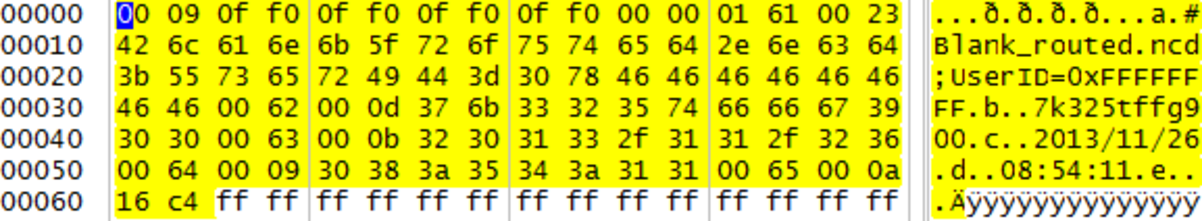
\includegraphics[width=0.75\textwidth]{fig/c3_desenvolvimento/ex3/hex_blank.pdf}
\caption{Cabeçalho do arquivo binário gerado no primeiro experimento para a configuração vazia.}
\label{fig:ex3:hex_blank}
\end{figure}

O cabeçalho é formado por chaves e tamanhos, indicando os diversos campos deste.
Ele contém pelo menos duas informações muito interessantes: o identificador do dispositivo alvo, que permite verificar a compatibilidade entre a configuração e o dispositivo que a está recebendo, e o tamanho da configuração, que permite que ela seja carregada de forma dinâmica sem necessidade de mais informações.

Na tabela \ref{tab:ex3:hex_blank} pode-se observar os tamanhos e campos apresentados na figura \ref{fig:ex3:hex_blank} \footnote{\qti{FAQ: Tell me about the format of the .BIT files please}, \url{http://www.fpga-faq.com/FAQ_Pages/0026_Tell_me_about_bit_files.htm}}.

\begin{table}[htp]
\centering
\begin{tabular}{cp{4cm}p{7.5cm}}
Tamanho & Chave & Significado\\ \hline
2 bytes & 9 (0x00 09) & Tamanho em bytes do próximo campo \\ \hline
9 bytes & 0x0f f0 0f f0 0f f0 0f f0 00 & Indica que a configuração a seguir é válida. \\ \hline
2 bytes & 1 (0x00 01) & Tamanho em bytes do próximo campo\\ \hline
1 byte & "a" (0x61) & Indica que os próximos campos conterão informações sobre o projeto e sobre a configuração. \\ \hline
2 bytes & 35 (0x00 23) & Tamanho em bytes do próximo campo \\ \hline
35 bytes & Blank\_routed.ncd;\qquad UserID=0xFFFFFFFF & Apresenta o nome do \textit{netlist} e o identificador do usuário. 0x00 ao final indica o final da string. \\ \hline
1 byte & "b" (0x62) & Indica que o próximo campo é um indentificador do dispositivo-alvo. \\ \hline
2 bytes & 13 (0x00 0d) & Tamanho em bytes do próximo campo \\ \hline
13 bytes & 7k325tffg900 & Identificador do dispositivo-alvo. 0x00 ao final indica o final da string. \\ \hline
1 byte & "c" (0x63) & Indica que o próximo campo é a data de sintese da configuração. \\ \hline
2 bytes & 11 bytes (0x00 0b) & Tamanho em bytes do próximo campo \\ \hline
11 bytes & 2013/11/26 & Data da síntese da configuração. \\ \hline
1 byte & "d" (0x64) & Indica que o próximo campo é a hora de síntese da configuração. \\ \hline
2 bytes & 9 bytes (0x00 09) & Tamanho em bytes do próximo campo \\ \hline
9 bytes & 08:54:11 & Hora de síntese da configuração. \\ \hline
1 byte & "e" (0x65) & Indica que os próximos 8 bytes contém o tamanho da configuração. \\ \hline
4 bytes & 661188 (0x00 0a 16 c4) & Tamanho em bytes da configuração a partir desta posição. \\\hline
\end{tabular}
\caption{Descrição do cabeçalho dos arquivos binários.}
\label{tab:ex3:hex_blank}
\end{table}

Existe ainda no cabeçalho 32 bytes de espaçamento preenchidos por com \qt{0xff} e bytes para autodetecção de largura de banda \cite{ug470, xapp583}.
Estes bytes (\qt{0x00 00 00 bb 11 22 00 44}) são usados no modo de configuração paralela para detectar automaticamente a largura de banda do arquivo de configuração.
O modo serial ignora todos os bits anteriores a palavra de sincronia \cite{xapp583}.
Estes bits são então usados apenas para pré-processamento do arquivo binário.

A palavra de sincronia (\qt{0xaa 99 ff 66}), encontrada a seguida, serve para indicar o inicio da configuração proprimamente dita e para alinhar o fluxo de dados nos registradores internos.

\subsection{Inicialização da Memória SPI Flash}
\label{sec:flash_indireta}
A memória SPI Flash, assim como todas as outras, precisa de um procedimento especial para poder ser inicializada com informações arbitrárias \cite{xapp694}.
Em geral, as únicas informações que podem ser gravadas nas memórias não-voláteis são configurações para o FPGA e programas para algum MicroBlaze embarcado \cite{ug111}.
Este processo é conhecido como programação indireta da memória Flash \cite{xapp586}.

\subsubsection{Compilação} Para a realização da programação indireta, o arquivo binário precisa ser compilado de forma a gerar um padrão de bits compatível.
Este procedimento é realizado na etapa de construção do processador.
Quando não especificado, o arquivo binário gerado utiliza a interface QSPI x1, que possui banda de transferência de 1 bit por leitura/escrita,  e relógio de frequência 3 MHz.
Com estas configurações, a programação do sistema demora apenas 1 minutos e 30 segundos \cite{xapp586}, mas pode ser ainda mais reduzido.

No PlanAhead, as configurações de compilação podem ser modificadas através do arquivo \qt{bitgen.ut} localizado na pasta \qt{etc} do projeto.
Através da opção \qt{-g SPI\_buswidth:X}, onde X pode ser 1, 2 ou 4, pode-se alterar a interface utilizada neste tipo de programação \cite{ug628, xapp576}, sendo a x4 a mais eficiente.
Pode-se ainda forçar a opção \qt{-g ConfigRate\_en:Y}, onde Y pode ser 3, 6, 9, 12, 16, 22, 26, 33, 40, 50 ou 66, para se utilizar de relógios de variadas frequências e obter assim o modo de configuração mais adequado para a memória em questão \cite{xapp586, ug628, ug810}.
Existe também a opção \qt{-g SPI\_Fall\_Edge:Yes}, que permite melhora margens de tempo e pode aumentar as taxas de leitura para configurações \cite{ug628, ug586}.
Uma opção alternativa é utilizar um relógio externo através da opção \qt{-g ExtMasterCclk\_en:Z}, onde Z pode ser \qt{Disable}, \qt{div-8}, \qt{div-4}, \qt{div-2} e \qt{div-1}.

\subsubsection{Arquivo de Memória PROM}
Após compilado o projeto, seu arquivo binário e qualquer outra informação a ser programada na memória Flash precisa ser adicionada a um arquivo do tipo MCS.
Este processo é necessário para que o iMPACT consiga carregar e programar a memória Flash de forma correta.
Pode-se construir este arquivo de memória PROM através do próprio iMPACT, processo que será descrito mais a frente.

\section{Experimento}
O teste deste experimento compreende a construção de um sistema microprocessador que carregue os arquivos binários da memória SPI Flash para a memória DDR3.
Este experimento contribuirá para a compreenção do processo de inicialização de memórias não-voláteis e do tratamento do cabeçalho dos arquivos binários.
Usará-se os programas XPS, SDK, que fazem parte do Embedded Development Kit (EDK), data2mem e iMPACT.

\subsection{XPS}
Utilizou-se o mesmo microcontrolador MicroBlaze construido no experimento passado, não sendo necessária nenhuma modificação.
A interface SPI utilizada aqui foi a padrão, x1, por motivos de simplificação do projeto.
O uso de uma interface x4 diminuiria o tempo de programação em 4 vezes, o que não é fator crítico para este experimento, mas acarretaria na necessidade de recompilar todos os projetos desenvolvidos até agora.

\subsection{SDK}
Logo após a construção do microcontrolador, recomenda-se construir o projeto do programa embarcado.
O procedimento para o SDK nesse caso é bem semelhante ao dos experimentos anteriores, mudando-se apenas os arquivos importados e a geração do \textit{linker script}.
Os arquivos a serem importados podem ser encontrados no CD de anexos.

O projeto do bootloader consiste apenas de uma máquina de estados para ler o cabeçalho do arquivo binário e interfaces com os drivers controladores das memórias DDR3 e SPI Flash e da interface de comunicação através da porta UART.

Desta vez, tem-se como objetivo fazer com que o sistema se carregue e entre em funcionamento de forma autônoma.
Para isto, precisa-se, depois da inclusão dos devidos arquivos, presentes no anexo, gerar o \textit{linker script}.
Este arquivo descreve como o arquivo binário do \textit{bootloader} deve ser armazenado na memória interna do FPGA para execução.
Este \textit{script} pode ser gerado clicando-se com o botão direito sobre o projeto do prgrama embarcado e selecionando-se a opção \qti{Generate Linker Script...} ou selecionando-se o projeto, abrindo-se o menu \qti{Xilinx Tools} e selecionando-se a opção do mesmo nome.
Para o escopo deste experimento, as configurações apresentadas na janela que se abre são suficientes, bastando clicar em \qti{Generate}.
A criação deste \textit{script} permite agora que se utilize o programa \qt{data2mem} para construir um arquivo binário de configuração com um programa embarcado pré-programado.

\subsection{data2mem}
A ferramenta data2mem funciona através da linha de comando, mas normalmente é acionada através de programas com interfaces gráficas, tais como o ISE, o XPS, o SDK e o iMPACT \cite{ug658}.
Sua função principal é o de mapear blocos contíguos de dados entre múltiplas \textit{Block RAMs} distribuídas pelo FPGA mantendo um acesso lógico contínuo, i.e., dados em endereços de memória adjacentes podem estar em blocos completamente diferentes.
No caso em questão, ela mapeará o \textit{bootloader} desenvolvido nas \textit{Block RAMs} de forma que no momento da programação, o MicroBlaze embarcado já possua um programa carregado.

Um comando típico do data2mem é construído com as opções \qt{-bm} para indicar o caminho para o arquivo do tipo \qti{Block RAM Memory MAP} (BMM), \qt{-bt} para indicar o caminho para o arquivo binário do tipo BIT, \qt{-bd} para indicar arquivos de programas do tipo ELF ou MEM, permitindo a inclusão de um identificador para associá-lo a algum dispositivo implementado, e \qt{-o b} para indicar o caminho do arquivo binário (BIT) de saída.
Um exemplo de uso do comando é apresentado abaixo.
\begin{lstlisting}[style=customVHDL]
data2mem \
-bm SDK/XPS_QSPI_Final_hw_platform/system_bd.bmm \
-bt SDK/XPS_QSPI_Final_hw_platform/system.bit \
-bd SDK/bootloader/Release/bootloader.elf tag microblaze_0 \
-o b SDK/XPS_QSPI_Final_hw_platform/download.bit
\end{lstlisting}

O comando acima também pode, como foi dito anteriormente, ser executado através do SDK.
Para isto, deve-se acessar o menu \qti{Xilinx Tools} e selecionar a opção \qti{Program Flash}.
Uma janela aparece, onde deve-se selecionar os arquivos BIT e BMM gerados pelo XPS na compilação do sistema e o arquivo ELF gerado na compilação do programa embarcado.
Este procedimento pode ser feito com a placa de desenvolvimento conectada ou não, gerando um erro que pode ser desprezado quando ela estiver desconectada.
O arquivo gerado pode ser encontrado na pasta \qt{SDK/*\_hw\_platform} sob o nome \qt{download.bit}.

\begin{figure}[htp]
\centering
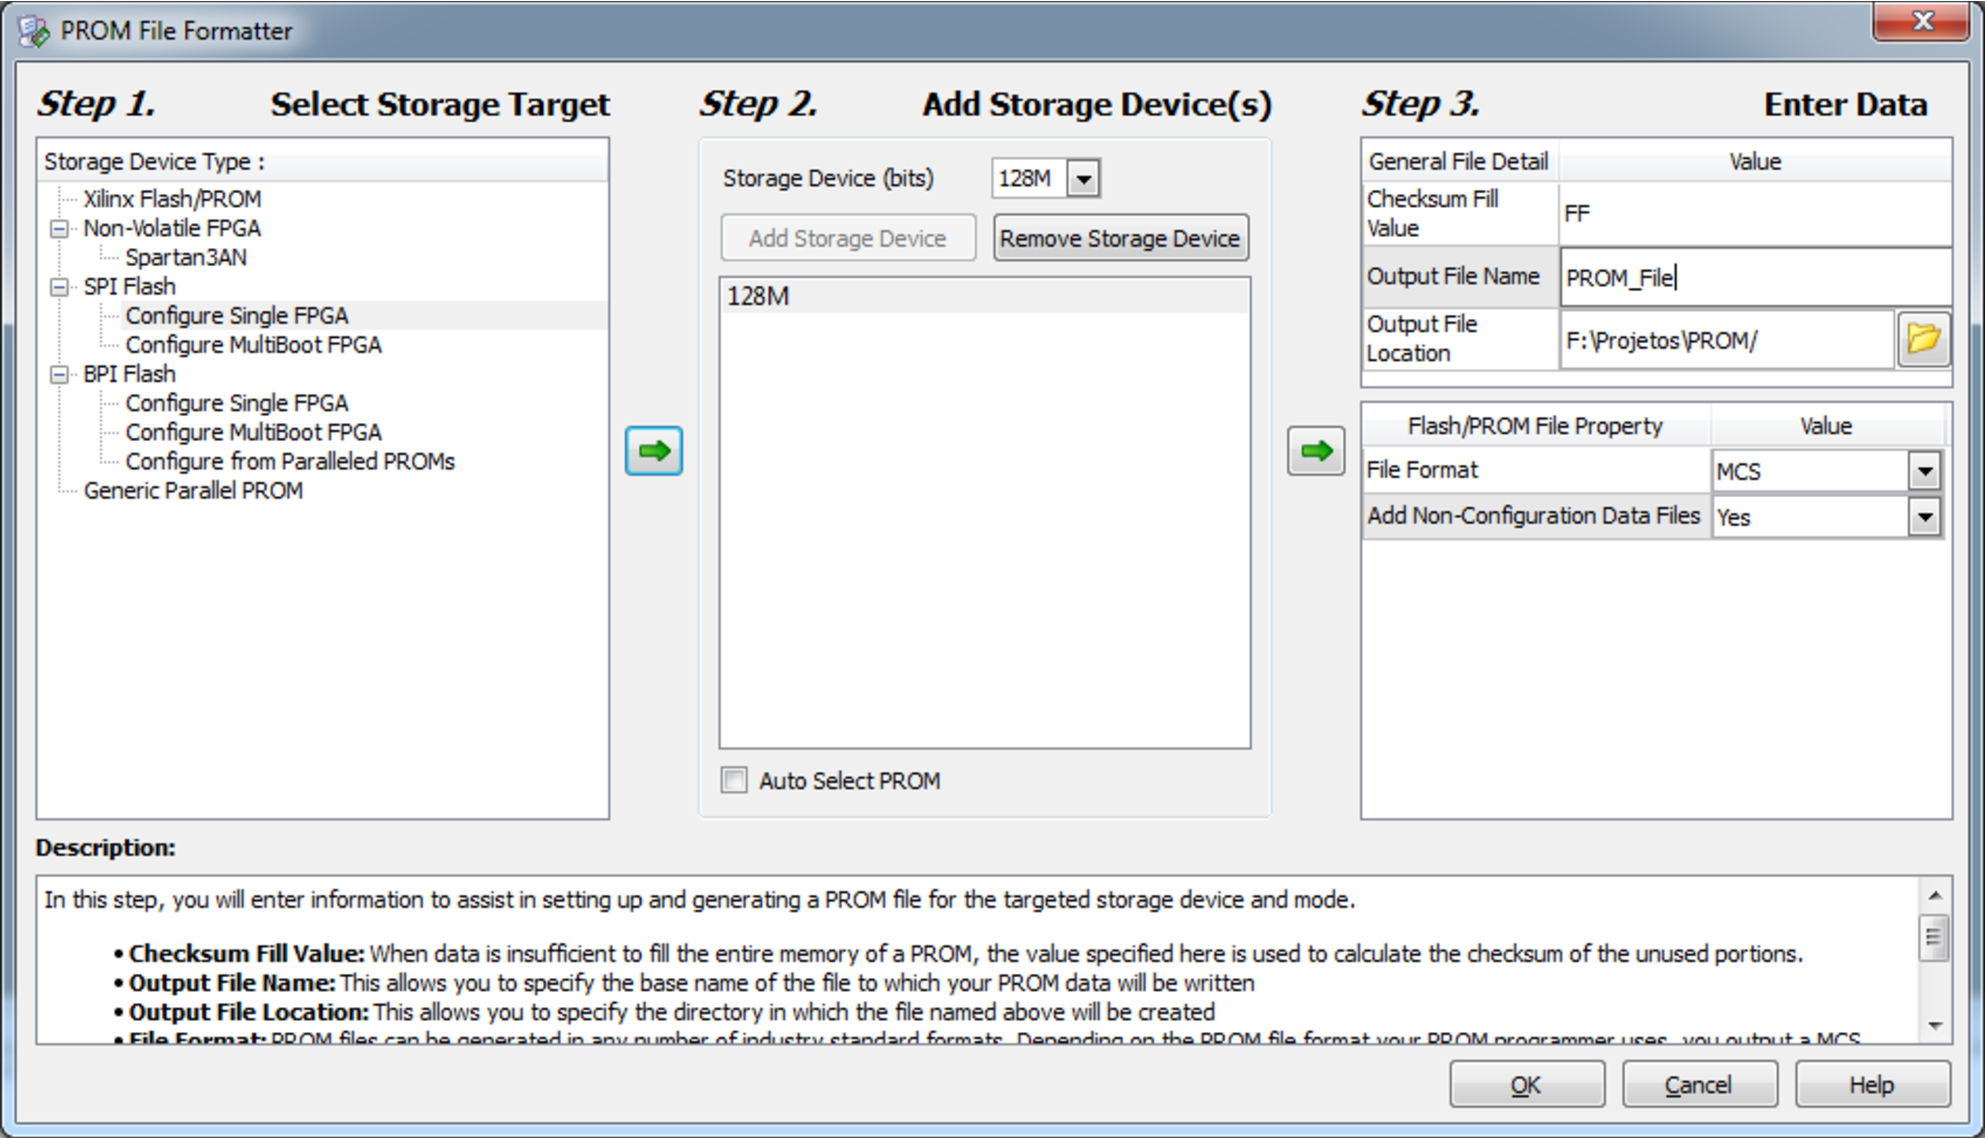
\includegraphics[width=0.9\textwidth]{fig/c3_desenvolvimento/ex3/PROM_File.pdf}
\caption{Janela para criação de um arquivo de memória PROM com as configurações devidamente ajustadas.}
\label{fig:ex3:prom_file}
\end{figure}

\subsection{Programação Indireta da Memória Flash}
Como todos os arquivos binários prontos, pode-se começar o processo de programação indireta da memória Flash.
Este processo se inicia através da criação de um arquivo de memória PROM através da ferramenta iMPACT.
Vale salientar apenas que faz-se necessário que todos os elementos (configurações totais e parciais) sejam previamente compilados para uma mesma interface SPI, seja ela x1, x2 ou x4.
O uso de interfaces diferentes pode gerar erros durante a programação da memória Flash.

No momento da criação do novo projeto do iMPACT, seleciona-se a opção \qt{\textit{Prepare a PROM File}}.
Na janela seguinte, seleciona-se \qti{SPI Flash/Configure Single FPGA} no primeiro painel e \qt{128M} no segundo e modifica-se \qti{Add Non-Configuration Data Files} para \qt{Yes}, conforme mostrado na figura \ref{fig:ex3:prom_file}.

Em seguida, adicionam-se os arquivos binários que se deseja programar na memória Flash.
O primeiro arquivo a se adicionar é o de configuração total.
Este arquivo é carregado durante o procedimento de inicio do FPGA.
Apenas um arquivo deste tipo precisa ser carregado neste experimento, apesar de ser possível realizar um projeto com diversas revisões de configurações ou múltiplas possibilidades de configurações de \textit{boot} \cite{xapp468, xapp1100}.
Para rejeitar a adicão de outras configurações, deve-se clicar em \qti{No} na mensagem de título \qti{Add Device}.

\begin{figure}[htp]
\centering
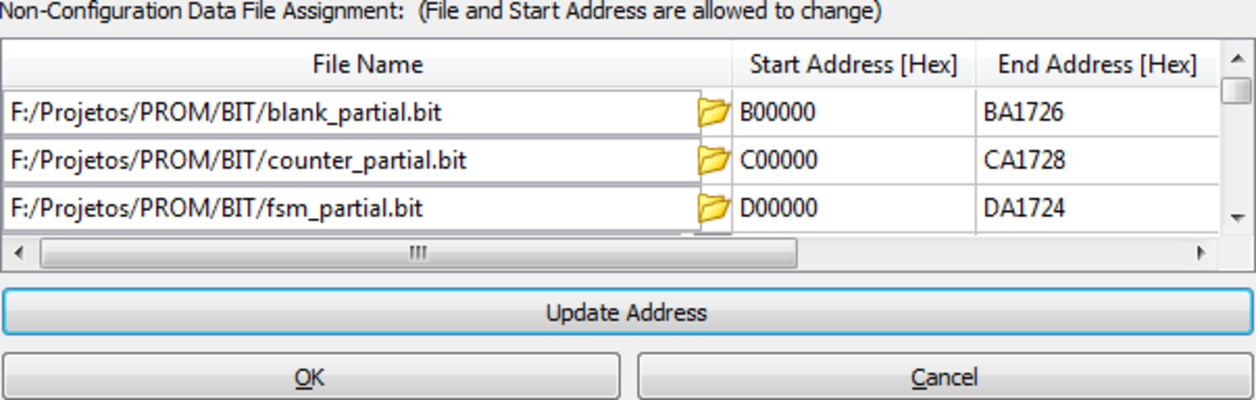
\includegraphics[width=0.75\textwidth]{fig/c3_desenvolvimento/ex3/PROM_Addr.pdf}
\caption{Janela para criação de um arquivo de memória PROM com as configurações devidamente ajustadas.}
\label{fig:ex3:prom_addr}
\end{figure}

A mensagem seguinte, \qti{Add Data File}, faz referência a adição de arquivos de dados neste projeto.
Clicando-se em \qti{Yes}, uma janela aparece com informações de endereçamento.
Pode-se aceitar os valores iniciais.
Estes arquivos podem ter qualquer conteúdo, mas o programa espera arquivos gerados pelo SDK, sendo necessário mudar a configuração de arquivos apresentados para \qti{All Files (*.*)}.
Após adicionar-se todos os arquivos, deve-se clicar em \qti{No} na janela de inclusão de novos arquivos de dados.
Ao se fazer isto, uma janela para indicação dos endereços é mostrada.
Recomenda-se mudar os endereços de início (\qti{Start Address}) para valores arredondados, como 0xB00000, 0xC00000 e 0xD00000, obedecendo os endereços das revisões, de forma a facilitar o trabalho de programação do sistema embarcado.
O botão \qti{Update Address} deve ser clicado para ajustar os endereços de fim (\qti{End Address}) antes de se prosseguir, obtendo-se algo similar a figura \ref{fig:ex3:prom_addr}.
Note que é possível incluir também um programa para o MicroBlaze na memória Flash, a ser carregado em tempo de execução, para controlar a mudança de configurações.

O último passo é gerar o arquivo, o que pode ser feito através do menu \qti{Operations} ou do painel \qti{iMPACT Processes}, selecionando-se a opção \qti{Generate File...}.
Este processo é rapido e resulta em um arquivo MCS gerado na pasta destino definida no passo da figura \ref{fig:ex3:prom_file}.

\section{Resultados}
Logo após a programação e após cada ciclo de energia (\textit{power cycle}), o programa embarcado envia dados da sua execução através da porta UART para o computador, gerando a saída mostrada na figura \ref{fig:ex3:resultado}.
Pode-se observar que o programa foi executado perfeitamente.

Note que a programação da FPGA através do iMPACT demorou sempre entre 800 e 1200 segundos, ou seja, entre 13 e 20 minutos, independente da largura de banda utilizada da interface utilizada.
O motivo para esta demora não é informado, mas suspeita-se que seja devido a velocidade de transmissão da porta JTAG ou devido a velocidade de escrita na memória SPI Flash.

\section{Conclusão}
O experimento realizado funcionou como esperado, tendo carregado as informações do computador para a memória Flash e, em tempo de execução, da memória Flash para a memória DDR3.
Ainda foi possível interpretar o cabeçalho do arquivo binário, extraindo dele informações importantes para o correto carregamento das configurações.
O processo de programação da memória Flash através do computador é bem demorado, chegando a levar 20 minutos, mas durante o \textit{boot} do sistema, ele é bem rápido, demorando apenas alguns poucos segundos.

É relativamente complicado trabalhar com os periféricos e \textit{drivers} que os acompanham devido a documentação escassa e a grande disperção das informações.
Este experimento só pode ser realizado devido a uma imensa pesquisa e compilação de guias de usuário, relatórios de aplicações, \textit{datasheets}, exemplos de projetos para diversos tipos de kits de desenvolvimento e comentários em fóruns de discussão.

\begin{figure}[htp]
\centering
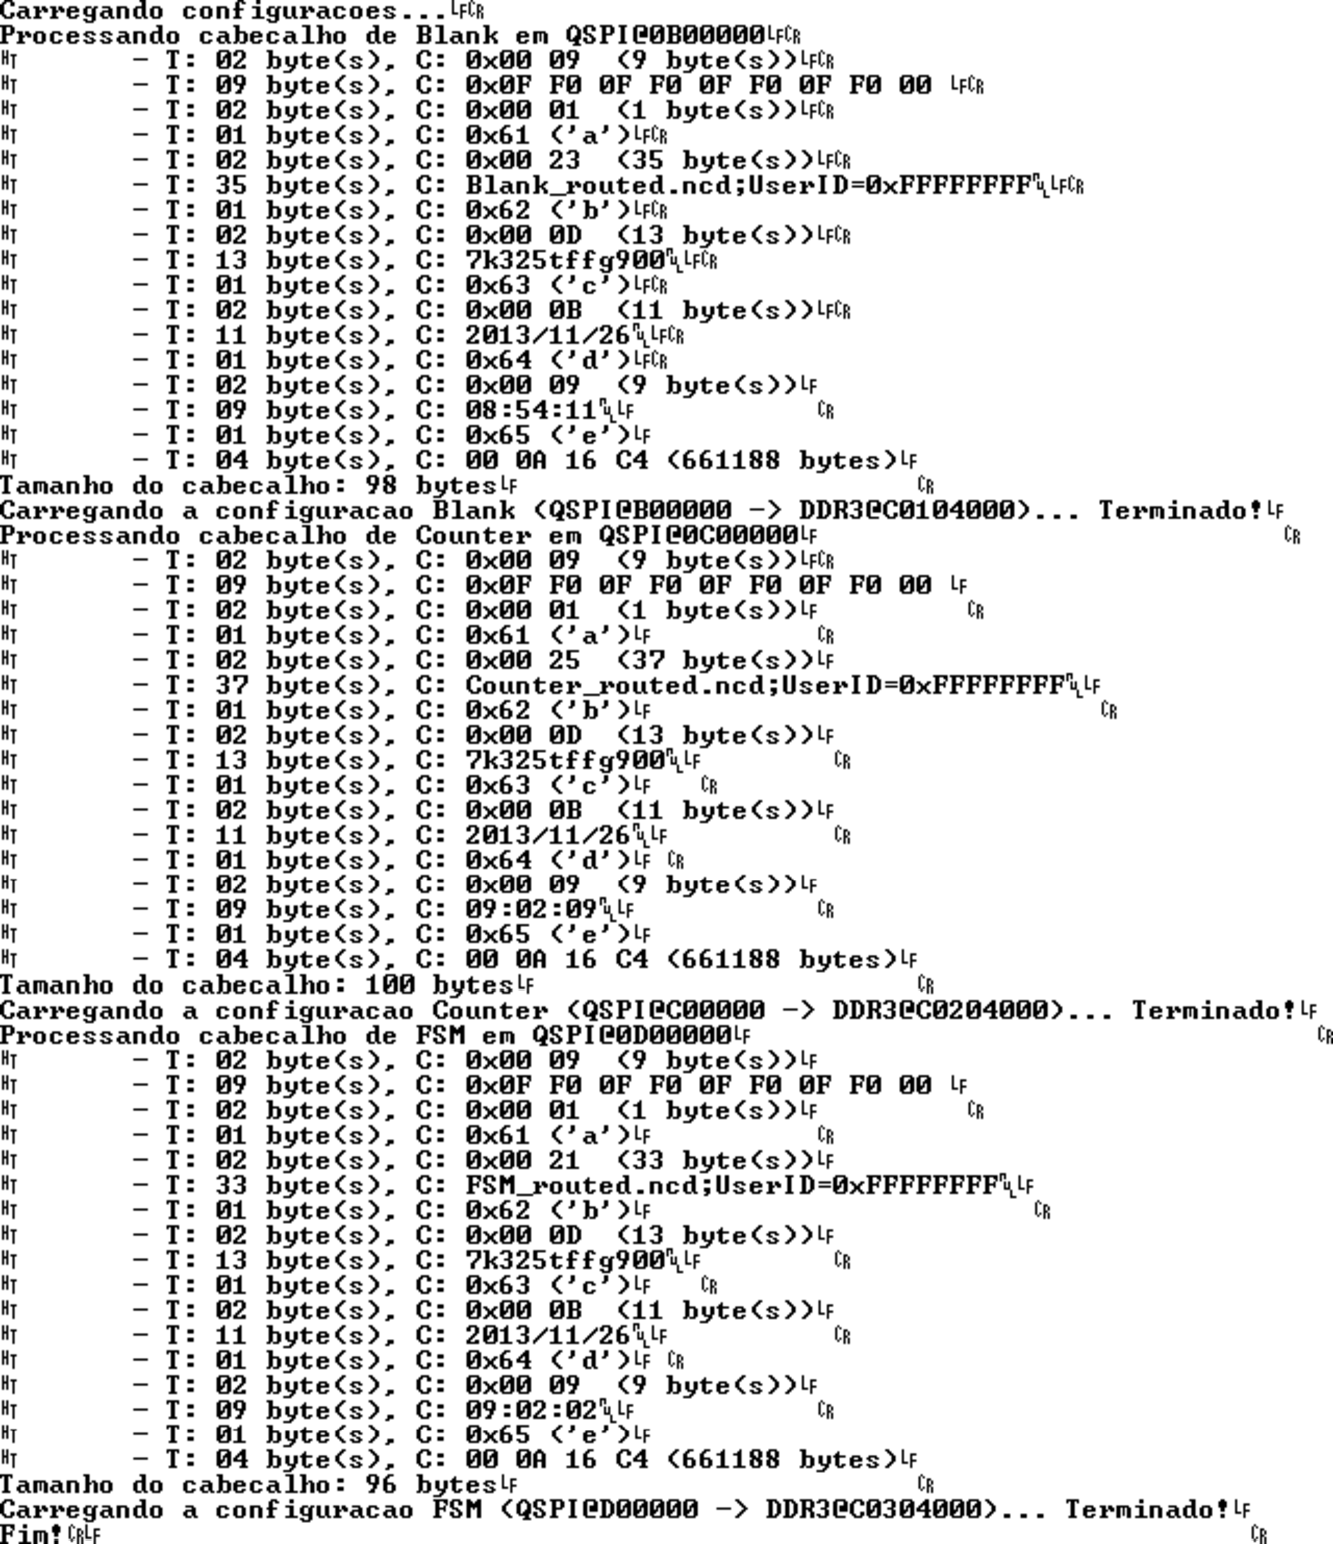
\includegraphics[width=0.8\textwidth]{fig/c3_desenvolvimento/ex3/Resultado_UART.pdf}
\caption{Resultado da execução do programa embarcado gravado na memória QSPI Flash.}
\label{fig:ex3:resultado}
\end{figure}

%%%%%%%%%%%%%%%%%%%%%%%%%%%%%%%%%%%
%					 Experimento 4
%%%%%%%%%%%%%%%%%%%%%%%%%%%%%%%%%%%

\chapter{Experimento 4 - Autoreconfiguração com \textit{MicroBlaze}}
Espera-se neste experimento projetar e implementar um sistema baseado em MicroBlaze que se reconfigure de forma autônoma, ou seja, sem a necessidade nenhum comando externo adicional.
Para isto, deve-se entender o funcionamento de alguns periféricos e seus \textit{drivers}, como integrar tudo de forma satisfatória, e o fluxo de projeto que permita as funcionalidades desejadas.

\section{Introdução Teórica}
O projeto em questão pretende utilizar um microcontrolador para acionar a troca de comportamentos de uma partição reconfigurável totalmente independente.
Tal feito pode, em teoria, ser alcançado facilmente através do periférico AXI4 HWICAP, que acessa as portas de configuração ICAP e ICAPE2, descritas a seguir.

\subsection{ICAP e ICAPE2}
As interfaces ICAP e ICAPE2 (\textit{Internal Configuration Access Port}) são formas de se acessar, tanto para leitura quanto para escrita, a configuração interna do FPGA.
Algumas das aplicações mais comuns que a utilizam incluem sistemas \textit{MultiBoot} \cite{xapp468, xapp1100}, sitemas frequentemente atualizados e sistemas críticos que necessitam de frequente verificação do correto funcionamento do sistema \cite{xapp468, xapp887}, e.g. sistemas embarcados em aplicações espaciais sucetíveis a radiações capazes de alterar o conteúdo dos elementos lógicos. 
Estas portas de configuração se utilizam de um protocolo identico ao da interface SelectMAP \cite{wp374, ug702}, que se utiliza de uma série de comandos para iniciar um dos vários procedimentos de programação.
Felizmente utiliza-se o controlador AXI4 HWICAP \cite{ds817}, que permite o controle da ICAP e ICAPE2 através do MicroBlaze.

Estas interfaces, tanto a SelectMAP quanto as ICAP e ICAPE2, possuem um largura de banda de 32 bits e frequência máxima de operação de 100 MHz, permitindo uma taxa de tranferência de até 3.2 Gbps \cite{ug702}.
Esta taxa de transferência permite que configurações parciais como a do experimento 1 sejam programadas em apenas 1.65 milisegundos ($611288\text{ bytes }\cdot8\frac{\text{bits}}{\text{byte}}\div3.200.000.000\frac{\text{bits}}{\text{segundo}} = 0,00165 \text{ segundo}$).

A única diferença entre as interfaces ICAP e ICAPE2 é a ausência de um sinal de espera na segunda.
A ICAPE2, apesar de ter um comportamente mais determinístico no que diz respeito aos tempos de escrita e leitura, não está disponível para alguns dispositivos.
A série de FPGAs 7 possui suporte a ICAPE2.

\subsubsection{Inversão dos bytes}
A SelectMAP necessita de uma inversão na ordem dos bits de cada byte do arquivo de configuração \cite{xapp502}, incluindo a palavra de sincronia, mencionada na seção \ref{sec:binario}.
Esta inversão só é aplicavel no uso das interfaces Serial, SelectMAP, e por consequência ICAP e ICAPE2, e BPI \cite{ug470}.
Note que alguns tipos de arquivos sintetisados, como o MCS e o HEX, já podem ter estes bytes invertidos não sendo necessário invertê-los novamente.
Não foi encontrada uma explicação para esta inversão.

\subsection{Fluxo de Projeto}
Este projeto começará no \textit{Project Navigator}, onde se instanciarão os componentes importados do experimento 1.
O arquivo referente ao MicroBlaze, gerando através de ferramentas de auxílio a construção deste tipo de componentes, também será adicionado.
Note, porém, que o fluxo de projeto não pode ser determinado com precisão, como mostrado na figura \ref{fig:ex4:prsoftwareflow}.
Cada um dos passos ISE, SDK e XPS necessitam de arquivos que são gerados em um dos outros, tornando este projeto de implementação indefinida.

\begin{figure}[htp]
\centering
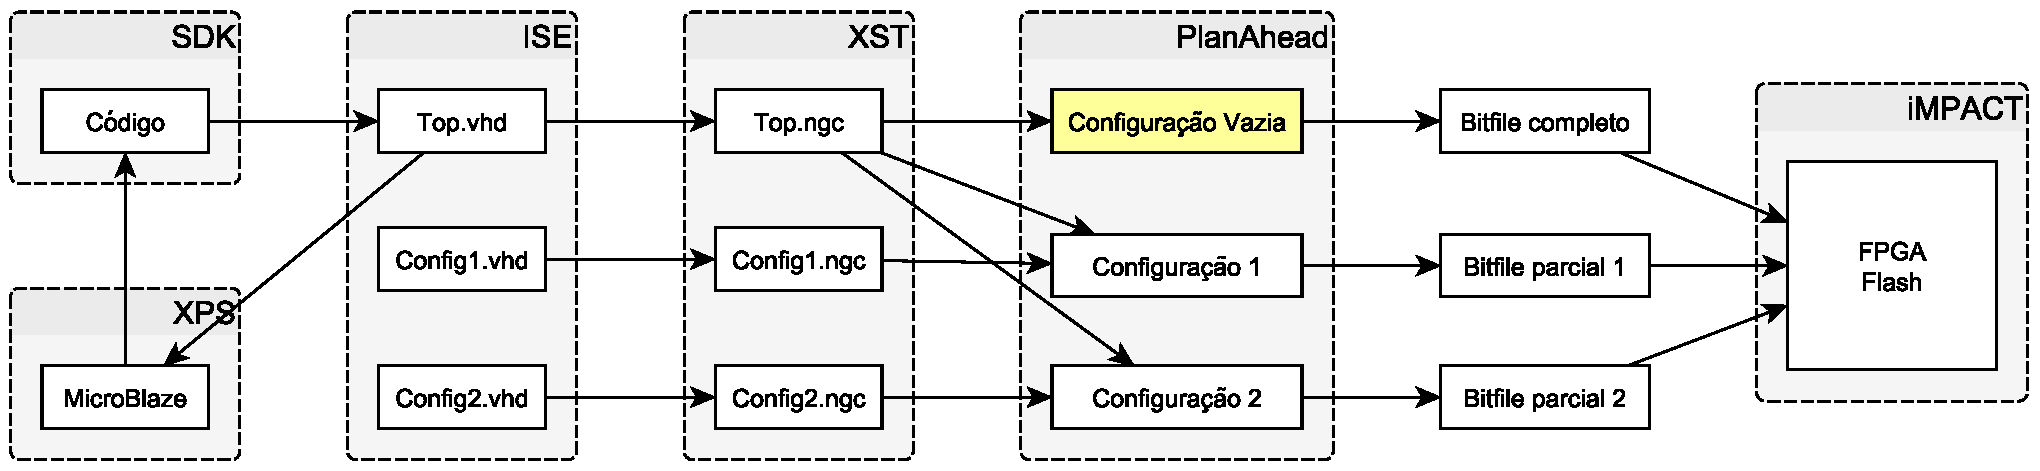
\includegraphics[width=0.95\textwidth]{fig/c3_desenvolvimento/ex4/prsoftwareflow.pdf}
\caption{Fluxo de ferramentas para desenvolvimennto do projeto.}
\label{fig:ex4:prsoftwareflow}
\end{figure}

Em busca por soluções, descobriu-se que é possível quebrar este ciclo através da construção manual de um arquivo de mapeamento de memória do tipo \textit{Block RAM}.
Sendo assim, o passo referente ao SDK não precisaria de informações do passo XPS.
Apesar disso, este passo possui um grau de complexidade muito elevado, além do escopo deste projeto.

\section{Resultados}
Este experimento foi abordado de diversas formas diferentes, mas nenhuma levou em nenhum resultado palpável.
Tentou-se implementar o microcontrolador com e sem memórias DDR3, visto que ela foi a causadora de diversos erros, mas até sem ela observou-se a necessidade de construção manual de arquivos complexos, processo impraticável considerando o escopo deste projeto.

\section{Conclusão}
Muitos erros e pouca documentação forçaram este experimento a ser considerado fracassado.
Sabe-se que sua realização não é impossivel, mas dadas as condições de tempo e conhecimento, deverá ser deixado de lado.

%%%%%%%%%%%%%%%%%%%%%%%%%%%%%%%%%%%
%					 Experimento 5
%%%%%%%%%%%%%%%%%%%%%%%%%%%%%%%%%%%

\chapter{Experimento 5 - Autoreconfiguração com \textit{MicroBlaze} 2}
Espera-se neste experimento projetar e implementar um sistema baseado em MicroBlaze que se reconfigure de forma autônoma, ou seja, sem a necessidade nenhum comando externo adicional.
Para isto, deve-se entender o processo de criação de periféricos reconfiguráveis e seus \textit{drivers}, o funcionamento do periférico AXI4 HWICAP e integrar tudo de forma satisfatória.

Ao contrário do experimento anterior, neste experimento não se utilizará o \textit{Project Navigator}, eliminando assim várias complexidades introduzidas por ele.

\section{Introdução Teórica}
O desenvolvimento de sistemas que suportem a autorreconfiguração ainda não é totalmente suportado pelas ferramentas da Xilinx, como foi mostrado no experimento anterior.
Algumas tarefas, como a inclusão de um executável em um processador (através do mapa de memória) instanciado em um sistema com módulos reconfiguráveis, precisam ser feitas a mão.
Apesar disso, as ferramentas suportam algumas outras opções, como a inclusão direta de um módulo reconfigurável como periférico em um microcontrolador.
Esta segunda opção será a abordada neste experimento.

\subsection{Periférico Reconfigurável}
A ferramenta XPS permite a construção de periféricos com comportamentos completamente arbitrários.
Estes periféricos podem ser utilizados para instanciar módulos reconfiguráveis \cite{ug744}.
O PlanAhead deve ser usado em conjunto com o XPS para a definição das partições e configurações.

\subsection{Fluxo do Projeto}
O projeto se inicia desenvolvendo a lógica do periférico reconfigurável, processo similar ao passo ISE nos experimentos anteriores.
Em seguida constrói-se o microprocessador utilizando este periférico.
Com o processador pronto, pode-se programá-lo, mesmo que ainda não possa testá-lo.
Por último, utiliza-se o PlanAhead para criar as diversas configurações e partições, sintetisando-as e implementando-as. 

\begin{figure}[htp]
\centering
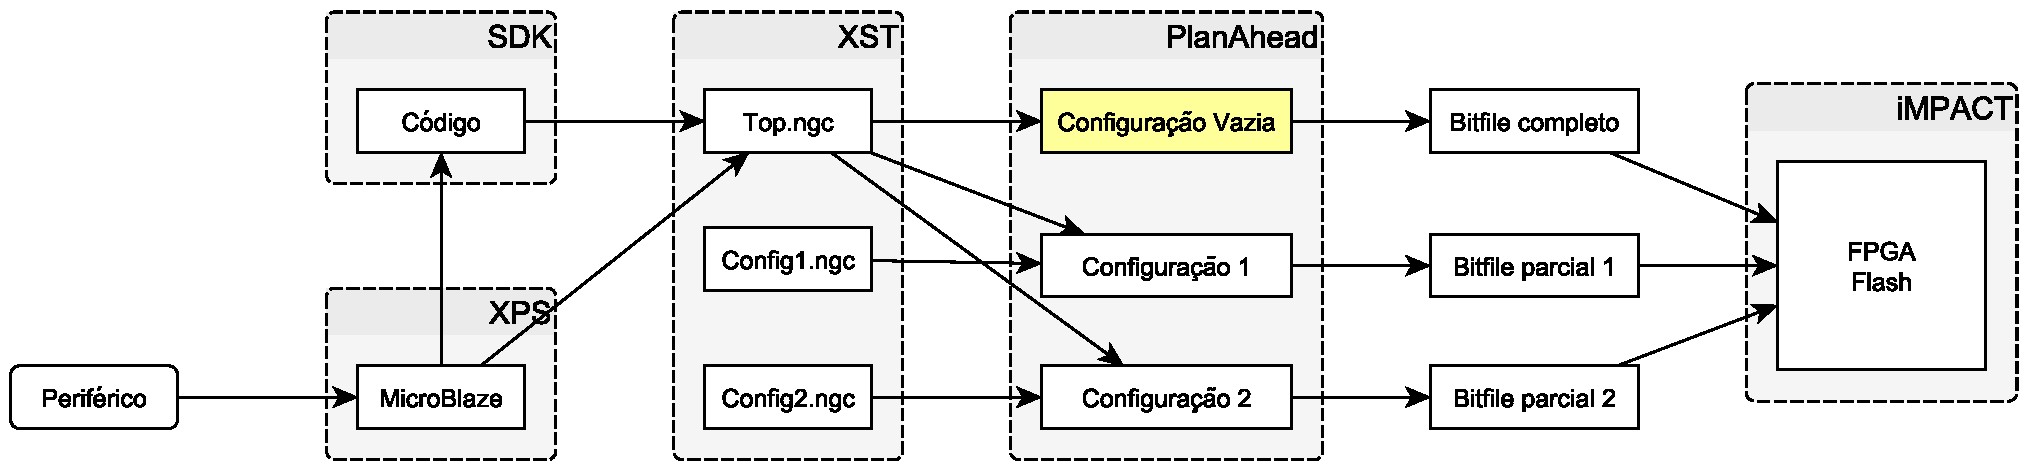
\includegraphics[width=0.95\textwidth]{fig/c3_desenvolvimento/ex5/prsoftwareflow.pdf}
\caption{Fluxo de ferramentas para desenvolvimennto do projeto.}
\label{fig:ex5:prsoftwareflow}
\end{figure}

\section{Experimento}
Este teste foi arquitetado para utilizar o máximo possivel dos elementos já desenvolvidos  neste trabalho.
Utilizará-se os comportamentos reconfiguráveis desenvolvidos no experimento 1 para a modelagem do comportamento do periférico reconfigurável, o microprocessador desenvolvido no experimento 2 sem a memória DDR3 e o programa desenvolvido no experimento 3 considerando a ausência da memória DDR3, para se construir um sistema microprocessado que possa acionar a mudança de configurações de uma partição reconfigurável.

\subsection{XPS}
Ao se abrir o programa, deve-se construir um sistema utilizando o BSB, assim como no experimento 2.
Quando questionado, seleciona-se os periféricos segundo a figura \ref{fig:ex5:perifericos}.
Note que a interface UART tem \textit{Baud Rate} de 115200 e o controlador da memória QSPI Flash tem modo de operação \textit{Quad}.

\begin{figure}[htp]
\centering''
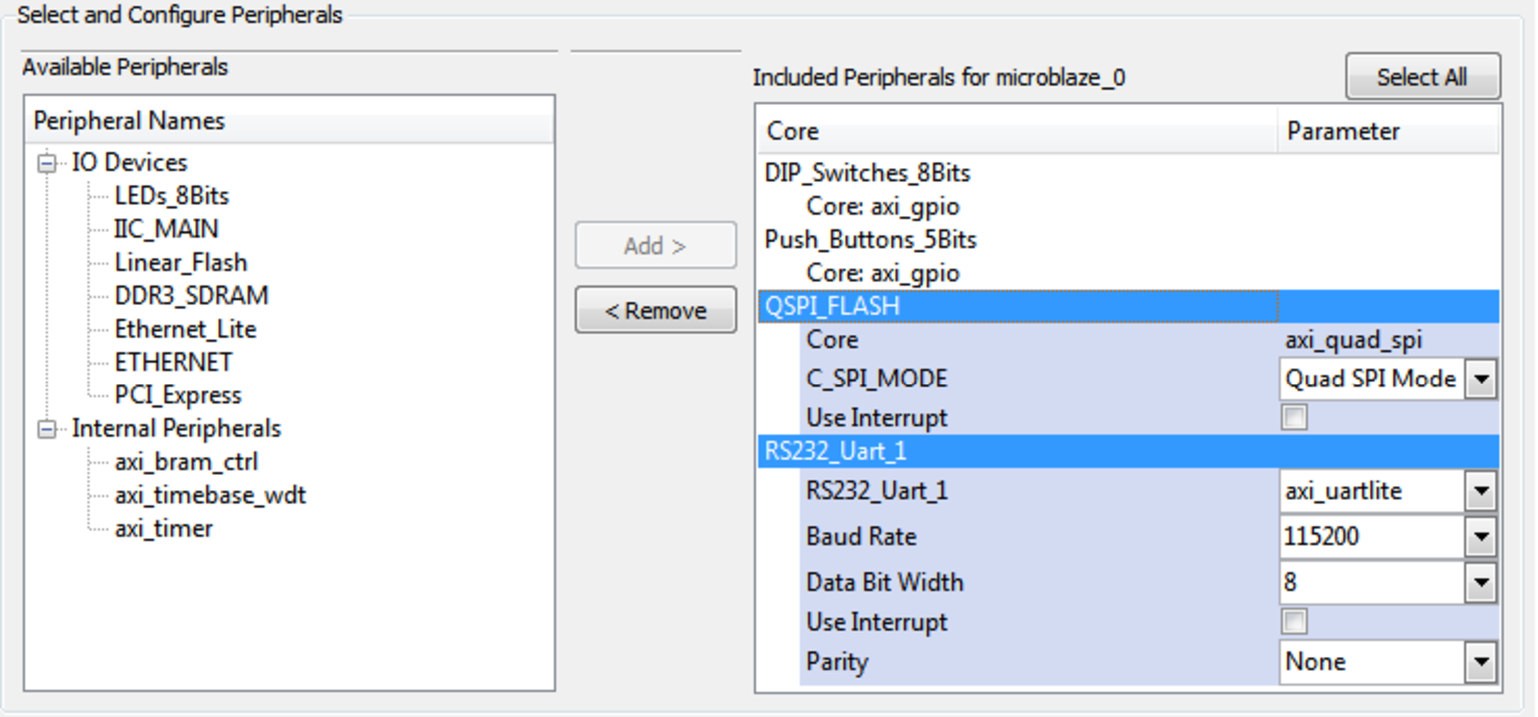
\includegraphics[width=0.95\textwidth]{fig/c3_desenvolvimento/ex5/perifericos.pdf}
\caption{Fluxo de ferramentas para desenvolvimennto do projeto.}
\label{fig:ex5:perifericos}
\end{figure}

Quando o programa termina de abrir, deve-se selecionar a opção \qti{Create or Import Peripheral...} do menu \qti{Hardware}.
Pode-se deixar todas as opções como estão, com excessão da \qti{Software reset} na página de \qti{IPIF (IP Interface) Services}.
Nota-se que foi criada a pasta \qt{pcores} com uma pasta com nome igual ao periférico recém criado.
Deve-se modificar os arquivos padrões criados para incluir a lógica do experimento 1.
Um exemplo de como se modificar este arquivo está presente no anexo.
Após modificado o periférico, deve-se reescanear a pasta de periféricos do usuário através da opção \qti{Rescan User Repositories} do menu \qti{Project}.
Em seguida pode-se adicionar este periférico ao sistema.

É necessário também a inclusão do periférico \qti{FPGA Internal Configuraion Access Port} (AXI\_HWICAP).
Na adição, deve-se marcar a opção \qti{Instantiate STARTUP primitive in the HWICAP core} para que o pino EOS (\textit{End of Startup}) não seja mais necessário.
Por causa disso é necessário também a mudança da opção \qti{Use Startup} para falso nas configurações da memória QSPI Flash.

É preciso ainda 

\subsection{XST}
\todo{XST}

\subsection{PlanAhead}
\todo{PlanAhead}

\section{Resultados}
\todo{Resultados}

\begin{lstlisting}
Slice Logic Utilization:
  Number of Slice Registers:                 2,820 out of 407,600    1%
    Number used as Flip Flops:               2,782
    Number used as Latches:                      3
    Number used as Latch-thrus:                  0
    Number used as AND/OR logics:               35
  Number of Slice LUTs:                      3,172 out of 203,800    1%
    Number used as logic:                    2,713 out of 203,800    1%
      Number using O6 output only:           2,084
      Number using O5 output only:             114
      Number using O5 and O6:                  515
      Number used as ROM:                        0
    Number used as Memory:                     339 out of  64,000    1%
      Number used as Dual Port RAM:            160
        Number using O6 output only:            96
        Number using O5 output only:             0
        Number using O5 and O6:                 64
      Number used as Single Port RAM:            0
      Number used as Shift Register:           179
        Number using O6 output only:           178
        Number using O5 output only:             1
        Number using O5 and O6:                  0
    Number used exclusively as route-thrus:    120
      Number with same-slice register load:    114
      Number with same-slice carry load:         6
      Number with other load:                    0

Slice Logic Distribution:
  Number of occupied Slices:                 1,553 out of  50,950    3%
  Number of LUT Flip Flop pairs used:        4,040
    Number with an unused Flip Flop:         1,473 out of   4,040   36%
    Number with an unused LUT:                 868 out of   4,040   21%
    Number of fully used LUT-FF pairs:       1,699 out of   4,040   42%
    Number of slice register sites lost
      to control set restrictions:               0 out of 407,600    0%
\end{lstlisting}

\section{Conclusão}

Observa-se que ainda é possível construir um sistema totalmente independente de microcontroladores, apesar de isto aumentar muito a complexidade do projeto.
Um bom balanço pode ser um sistema onde um MicroBlaze com um \textit{bootloader} está implementado em uma partição reconfigurável e pode ser apagado após o início do sistema, restando assim apenas entender o funcionamento da interface ICAP ou ICAPE2 e do controlador de DDR3 criado pelo MIG.

\ifx\compilewholereport\undefined
	\bibliographystyle{plain}
	\newsavebox\mytempbib\savebox\mytempbib{\parbox{\textwidth}{\bibliography{bibliografia}}}

	\listoftodos
	\end{document}
\fi